%\documentclass[12pt,titlepage]{report}
\documentclass{bakalarka}
\usepackage[utf8]{inputenc}
\usepackage[czech]{babel}
\usepackage{amsmath}
\usepackage{amsfonts}
\usepackage{amssymb}
\usepackage{microtype}
%\usepackage[Sonny]{fncychap}

\usepackage{algorithmicx}
\usepackage{algorithm}
\usepackage{algpseudocode}
\usepackage[justification=centering]{caption}

\usepackage{wrapfig} % testing
\usepackage{booktabs} % beautify tables?

\usepackage{chngpage}

\usepackage{graphicx}
\usepackage{epstopdf}

\usepackage{ae}
\usepackage{fancyhdr}

\usepackage{lscape} % horizontal tables
\usepackage{rotating}

\usepackage{tocloft}

\usepackage[left=3.5cm,right=2.5cm,top=4cm,bottom=.1cm]{geometry}

\usepackage[section]{placeins}

\usepackage[pdfborder=0 0 0]{hyperref}

%\usepackage[citestyle=numeric,url=true]{biblatex}
%\addbibresource{ref.bib}
\usepackage[numbers]{natbib}

\makeatletter
\renewcommand{\ALG@name}{Algoritmus}
\renewcommand{\listalgorithmname}{List of \ALG@name	s}
\makeatother

\author{Tomáš Maršálek}
\title{Měření významnosti autorů v citační síti}
\titlet{}
\titlett{}
\university{Západočeská univerzita v Plzni}
\faculty{Fakulta aplikovaných věd}
\department{Katedra informatiky a výpočetní techniky}
\subject{Bakalářská práce}
\town{Plzeň}

\begin{document}
\shorthandoff{-}
\pagestyle{fancy}

% \begin{titlepage}
% \begin{center}
% 	\Large{Západočeská univerzita v Plzni} \\
% 	\Large{Fakulta aplikovaných věd} \\
% 	\Large{Katedra infromatiky a výpočetní techniky} \\
% \mbox{} \\[1.6cm]
% 	\LARGE{{\bf Bakalářská práce}} \\
% \mbox{} \\
% 	\Huge{{\bf Měření významnosti autorů v citační síti}} \\
% \end{center}
% \vfill
% \begin{minipage}{.5\textwidth}
% Plzeň, 2013
% \end{minipage}
% \begin{minipage}{.5\textwidth}
% \hfill Tomáš Maršálek
% \end{minipage}
% \thispagestyle{empty}
% \end{titlepage}
\renewcommand{\chaptermark}[1]{\markboth{\textit{#1}}{}}
% \renewcommand{\sectionmark}[1]{\markrigth{\textit{#1}}{}}
\cfoot{\thepage}
\lhead{\leftmark}
\rhead{\rightmark}
\maketitle

\chapter*{Prohlášení}
\thispagestyle{empty}
Prohlašuji, že jsem bakalářskou práci vypracoval samostatně a výhradně s~použitím citovaných pramenů.
\vskip 0.7em
\hskip 9cm Tomáš Maršálek

\chapter*{Abstract}
\thispagestyle{empty}
% Prvky sociální sítě, které nemají žádné apriorní ohodnocení významnosti, jsou
% různě významné pouze na základě vztahů s okolními prvky. V této práci byly
% prozkoumány a implementovány známé metody centrality a bibliografické metody
% měřící významnost prvků v sociální nebo citační síti. Výsledky aplikování metod
% na volně dostupné citační databáze ukázaly vysokou podobnost jednotlivých metod
% a rovněž shodu nejvýznamnějších autorů dle těchto metod se známými oceněními v
% oblasti informatiky a informační vědy (Turing Award, Codd, ACM Fellows, ISI
% Highly Cited). Bylo zjištěno, že některé implementované metody jsou i přes
% použití nejrychlejších algoritmů výpočetně příliš náročné vzhledem k velikosti
% citačních sítí, vzniklých z těchto citačních databází. Dále bylo empiricky
% potvrzeno, že implementované metody měří významnost, byť může mít více
% interpretací.

%\listoffigures
%\listoftables
%\thispagestyle{empty}

\clearpage
\pagestyle{empty}
\setlength{\cftbeforetoctitleskip}{-2em}
\tableofcontents

\addtocontents{toc}{\protect\thispagestyle{empty}}
\clearpage
\setcounter{page}{1}
\pagestyle{fancy}
\chapter{Úvod}
V době, kdy je celý svět propojen internetem a sociálními sítěmi, si podvědomě
začínáme uvědomovat provázanost celého světa a všímáme si struktur kolem nás s
charakterem sítě. Úspěchem je rozpoznat síťovou strukturu a popsat ji, ale
můžeme jít s myšlenkou dál? Jaké informace zjistíme, pokud budeme blíže zkoumat
uzly a jejich spojení? V této práci nás bude zajímat jedna konkrétní
kvalitativní vlastnost uzlů - významnost.

Významnost není jednoznačně definována, ale intuitivně cítíme, pokud je
například člověk významný mezi svými přáteli nebo můžeme zjistit, které město
je klíčovým dopravním uzlem v železniční síti.  Představme si, že neznáme
jednotlivé lidi v síti přátel a žádné informace o nich. Jak zjistíme, kdo je
nejvýznamnější pouze na základě vztahů mezi nimi? Naším cílem je zjistit nejen,
které prvky obecné sítě jsou významné a které nikoliv, ale pokusíme se najít
metody, jak seřadit prvky od nejvýznamnějšího po nejméně významný.

Velký díl k zodpovězení otázky relativní významnosti prvků definovali
Freeman~\citep{freeman1979}; Bonacich~\citep{bonacich1972}, jehož práce je
spojena s Hubbellovo~\citep{hubbell1965} mírou sociometrického statusu;
Coleman~\citep{coleman1973} se svou mírou síly a Burt~\citep{burt1982} a jeho
míra prestiže~\citep{friedkin1991}. Významnost prvku bývá v sociální síti
označována jako centralita a metody pro zjištění centrality jsou známé jako
míry centrality (centrality measure). Původně byly vyvinuty v sociologickém
kontextu pro analýzu sociálních sítí, ale jejich princip lze snadno zobecnit na
obecný graf, proto můžeme využít těchto metod pro analýzu citačních nebo jiných
komplexních sítí, které nemají čistě sociologický význam.

Tato práce je věnována citačním sítím, ale používáme metody z analýzy
sociálních, dopravních, komunikačních a jiných sítí. V citační síti hledáme
nejvýznamnější autory pouze podle toho, jak jsou provázáni s jinými autory
podle referencí v publikacích, které vydali. Významnost autorů není úplnou
neznámou, protože existuje množství ocenění, která byla udělena právě významným
autorům a vědcům za jejich dílo. Samotné udělení ocenění mohlo tyto autory
udělat významnými, přestože předtím nebyli. V jiném případě mohlo být důležité
ocenění příčinou ještě větší významnosti autora. 

Budou přiblíženy detaily o nejpoužívanějších mírách centrality (degree,
eigenvector centrality, betweenness centrality, closeness centrality),
bibliografické metodě h-index a jejich implementaci. Výsledkem budou porovnání
jednotlivých metod aplikovaných na citační sítě vytvořené z citačních databází
DBLP a CiteSeer, které zároveň srovnáme s oceněními autorů v oblasti
informatiky (ACM SIGMOD Edgar F. Codd Innovations Award, ACM Fellows, ACM A.M.
Turing Award, ISI Highly Cited highlighted).

Cílem této práce je vytvořit knihovnu pro analýzu citační sítě s metodami pro
měření významnosti autorů, použít ji pro nalezení žebříčků nejvýznamnějších
autorůpro každou metodu. Tyto žebříčky poté mezi sebou porovnáme a jednotlivé
metody srovnáme s již udělenými oceněními. Očekáváme, že pokud měříme
významnost autora nebo obecně prvku v síti, přestože neznáme její přesnou
definici, bude se shodovat s těmito oceněními.

% TODO Nejsou již někde autoři oceněni za to jak jsou významní? 
% TODO Nutnost měřit významnost prvků sítě, v tutom případě autorů. I když jediná informace je jak jsou propojený. 
% TODO Byla proto vytvořena knihovna, která implementue zmíněné metody.
% TODO Metody budou porovnány mezi sebou a srovnány s oceněními, které se udělují významným autorům.
% TODO Navazuji na práci Nykla, Fialy a dalších autorů, který mam třeba v referencích.

\chapter{Sociální a citační sítě}

Myšlenka sociální sítě existovala dlouho předtím, než je pod tímto termínem
začali lidé rozpoznávat. Jedná se o komplexní struktury vztahů mezi členy
sociálních uspořádání na všech úrovních - od osobních až po mezinárodní vztahy
mezi organizacemi.

Nejčastěji se ale setkáme se sociální sítí jako strukturou tvořenou lidmi,
kteří jsou svázáni nějakým sociálním vztahem, zejména v poslední době s
rozmachem populárních webových sociálních sítí (MySpace, Facebook, G+, Lidé),
jím bývá přátelství.

\section{Reprezentace sítí}
Abychom mohli pracovat s doposud abstraktním konceptem sítě, musíme být schopni
ji reprezentovat jako datovou strukturu, na níž poté provedeme jakoukoliv
analýzu.
V odvětví matematiky teorie grafů je síť (graf) dvojice množin uzlů $V$
(vrcholů) a spojení uzlů $E$ (hran) $G = (V, E)$.  Obecně můžeme uvažovat grafy
s hranami s orientací či bez orientace. V obou případech se stále jedná o
dvojici $(V, E)$, pouze pro orientovaný graf je množina hran množinou
uspořádaných dvojic oproti množině neuspořádaných dvojic u neorientovaného
grafu.

V definici grafu je množina hran $E$ soubor dvojic, které označují koncové uzly
hrany, neboli jejich spojení. Samotné spojení je jediná informace, kterou
množina hran nese. Chceme-li zaznamenat nějakou další informaci, která je
spojená se spojením dvou uzlů, namísto hrany jako dvojice koncových uzlů,
nadefinujeme hranu jako n-tici, kde první dvě hodnoty jsou koncové uzly a zbylé
hodnoty nesou libovolnou informaci. Ve většině případů si vystačíme s jednou
dodatečnou informací a nazýváme ji váha hrany. Jiná možnost pro zavedení vah
hran je váhová funkce $f: E \mapsto \mathbb{R}$, kde $f(e) = w$ je ohodnocení
konkrétní hrany $e \in E$. V případě zavedení vah hovoříme o vážených sítích.

Při zavedení vah máme například možnost používat síť jako multigraf, tedy graf,
u kterého je povoleno více spojení mezi dvěma stejnými uzly. Počet stejných
hran pak pouze zaznamenáme celočíselnou hodnotou ve váze hrany.

Síť world wide web tvořená webovými stránkami je příkladem
multigrafu, protože je povoleno z jedné stránky odkazovat na jinou na více
místech. Při analýze takovýchto sítí využijeme právě vah hran a počet
hypertextových odkazů mezi dvěma stránkami zaznamenáme vyšším ohodnocením
hrany. V tomhle případě znamená vyšší váha silnější pouto mezi uzly.

Jiným případem může být např. síť, kde sledujeme města a dopravní spojení
mezi nimi. V tomto případě nás může zajímat vzdálenost nebo časová náročnost
na dopravu mezi dvěma městy, které budou znamenat silnější pouto, pokud budou
mít naopak menší váhu. Hledáme totiž nejkratší či nejrychlejší spojení.


Pro reprezentaci v paměti počítače se nejčastěji používají dva způsoby - matice
sousednosti a graf pomocí spojových seznamů.  Hrany se uzlu v případě
orientovaného grafu liší z pohledu jednoho uzlu. Pokud hrana vychází z tohoto
uzlu, nazveme ji výstupní hrana, v opačném případě se bude jednat o vstupní
hranu.


Matice sousednosti (adjacency matrix) je čtvercová matice $A$ o velikosti počtu
vrcholů grafu $|V|$, ve které prvek ${\bf A}_{uv}$ na řádku $u$ a sloupci $v$
určuje jestli existuje hrana od vrcholu $u$ do vrcholu $v$. Pokud je hodnota
${\bf A}_{uv}$ $1$, hrana existuje; pokud je hodnota $0$, pak hrana neexistuje
a pokud je hodnota $w$, pak hrana existuje s váhou $w$.

Jiným maticovým způsobem uchování grafu je incidenční matice ${\bf B}$.
Incidenční matice vyjadřuje vztah mezi vrcholy a hranami tak, že ${\bf B}_{ue}
= 1$, pokud vrchol $u$ je spojený s hranou $e$, a $0$ v opačném případě. V
orientovaném grafu rozlišujeme mezi počátečním uzlem ${\bf B}_{ue} = -1$ a
koncovým uzlem ${\bf B}_{ue} = 1$. Incidenční matice se pro výpočetní teorii
grafů často nepoužívá z důvodu paměťové náročnosti, která je pro většinu grafů
výrazně vyšší než u matice sousednosti ($\Theta(|V||E|)$ oproti
$\Theta(|V|^2)$, kde množina hran dosahuje velikostí $O(|V|^2)$).

Nejčastěji používáme myšlenku sousednosti vrcholů, ale namísto reprezentace
maticí, která je ve většině případů řídká a zbytečně obsahuje velké množství
nul, použijeme reprezentaci řídké matice - řádek nahradíme seznamem vrcholů,
které v matici sousednosti mají nenulovou hodnotu. Tento způsob je známý jako
graf pomocí spojových seznamů (adjacency list representation of a graph).


\section{Citační sítě}
Citační sítě jsou podobné sociálním sítím, pouze místo uzlů, které představují
osoby, se v citační síti jedná o publikace nebo autory těchto publikací. Pokud
je uzlem publikace, pak hrany této sítě symbolizují citaci publikace jinou
publikací. V druhém případě uvažujeme síť, kde uzly reprezentují autory knih,
vědeckých článků, vědecké literatury a dalších publikací. Prvnímu typu říkáme
síť publikací, druhému síť autorů. Citační sítě patří do kategorie bezškálových
sítí. Citační síť autorů pro databázi DBLP i CiteSeer mají mocninné rozložení
stupňů i vah hran (obr.~\ref{fig:dblpweightsdistribution}, \ref{fig:citeseerweightsdistribution}).

\subsection{Citační síť publikací}
Uvažujeme-li první případ, kde uzly reprezentují publikace a hrany přímo citace
mezi těmito publikacemi, jedná se o síť publikací. Pokud publikace $A$ odkazuje
na publikaci $B$, budou existovat stejnojmenné uzly $A$ a $B$ a hrana mezi
těmito uzly může mít dvě různé orientace podle svého uplatnění. Směr od
citující publikace k citované (v našem příkladě od $A$ do $B$) bude mít hrana,
kterou označíme jako výstupní pro uzel $A$ a vstupní pro uzel $B$.  Výstupní
hrana, laicky řečeno, označuje vztah \uv{cituji}, kdežto vstupní hrana znamená
\uv{jsem citován}.

\subsection{Citační síť autorů}
Druhou citační sítí je citační síť autorů. Zde je uzel reprezentací autora a
hrany spojují autory mezi sebou. Ve většině případech máme k dispozici data ve
formátu, který přímo odpovídá síti publikací, tj. pro každou publikaci známe
seznam jejích autorů a odkazů na další publikace. Síť autorů lze získat
transformací sítě publikací tak, že každou hranu z původní sítě publikací
přiřadíme každému z autorů citující publikace a duplikujeme ji pro každého z
autorů citované publikace (obr.~\ref{fig:transform}). Celkově vznikne $nm$ nových hran, pokud odkazovaná
publikace obsahuje $n$ autorů a odkazující $m$ autorů. Stejně jako v síti
publikací, i zde uvažujeme opačné orientace hrany.

\begin{figure}[!ht]
\begin{minipage}[b]{0.45\textwidth}
\centering
	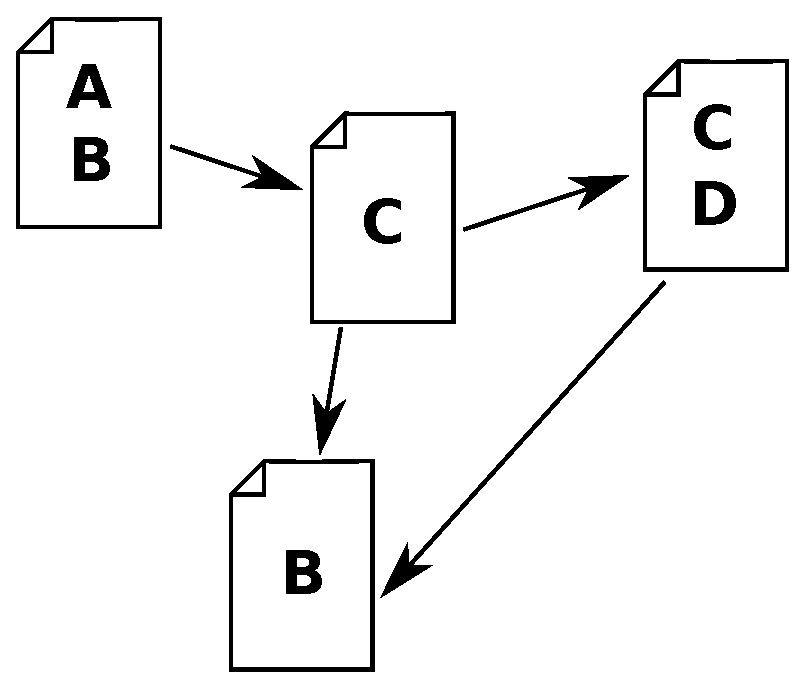
\includegraphics[width=\textwidth]{pubs.eps}
\end{minipage}
\hspace{0.5cm}
\begin{minipage}[b]{0.45\textwidth}
\centering
	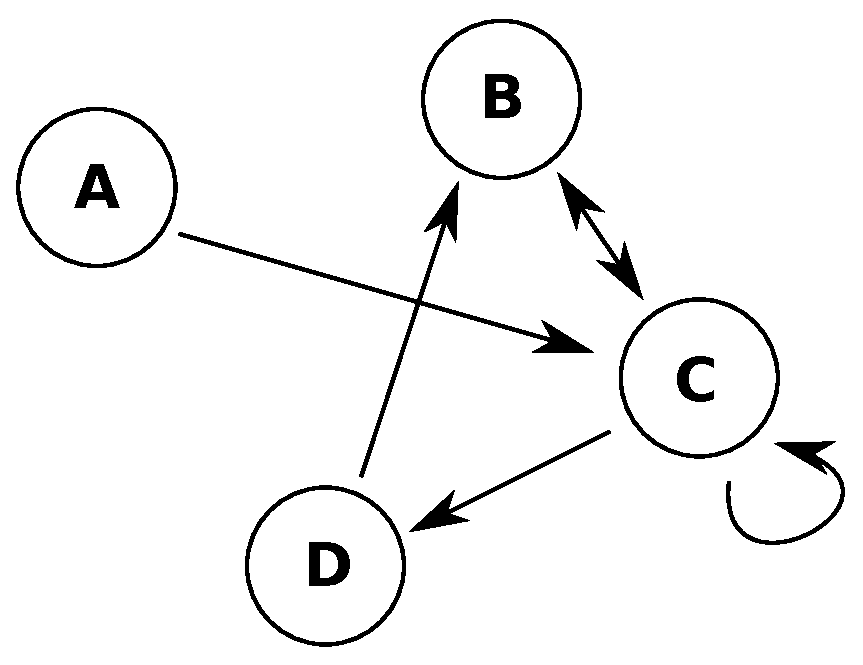
\includegraphics[width=\textwidth]{auths.eps}
\end{minipage}
\caption{Transformace z citační sítě publikací na citační síť autorů}
\label{fig:transform}
\end{figure}

V síti autorů má pro naše účely smysl uvažovat ohodnocení hran. Existuje více
způsobů, jak lze přiřadit ohodnocení (váhu) jednotlivým hranám, ale
nejjednodušším způsobem je prosté přiřazení počtu publikací, jejichž autorem je
daný autor $A$, které odkazují na publikace, jejichž autorem je autor $B$.

Druhou možností ohodnocení hran, který využívá implementovaná knihovna pro
některé metody, je převrácená hodnota prvního způsobu ohodnocení. Důvodem je
přímá souvislost mezi váhou hrany a vzdáleností mezi uzly. V prvním případě
(obr.~\ref{fig:wNormal}), kdy silnější pouto mezi autory vyjadřuje vyšší
ohodnocení hrany, v druhém případě (obr.~\ref{fig:wRecip}) je naopak nižší váha
vyjádřením silnějšího vztahu, jelikož jsou si uzly blíže.  Tento způsob je
používán pro algoritmy, které pracují na myšlence nejkratších cest mezi uzly. 

\subsection{Vážené citační sítě}
Pro citační sítě můžeme uvažovat ohodnocení hran obojího typu. Například mezi
dvěma autory může být silnější vztah, pokud se citují ve více publikacích.
Jestliže citační síť analyzujeme metodami, které jsou založené na myšlence
hledání nejkratších cest i v této síti, která nemá v podstatě žádný pojem
vzdálenosti, použijeme druhý typ ohodnocení - menší váha, silnější pouto.

\begin{figure}[!ht]
\begin{minipage}[b]{0.45\textwidth}
\centering
	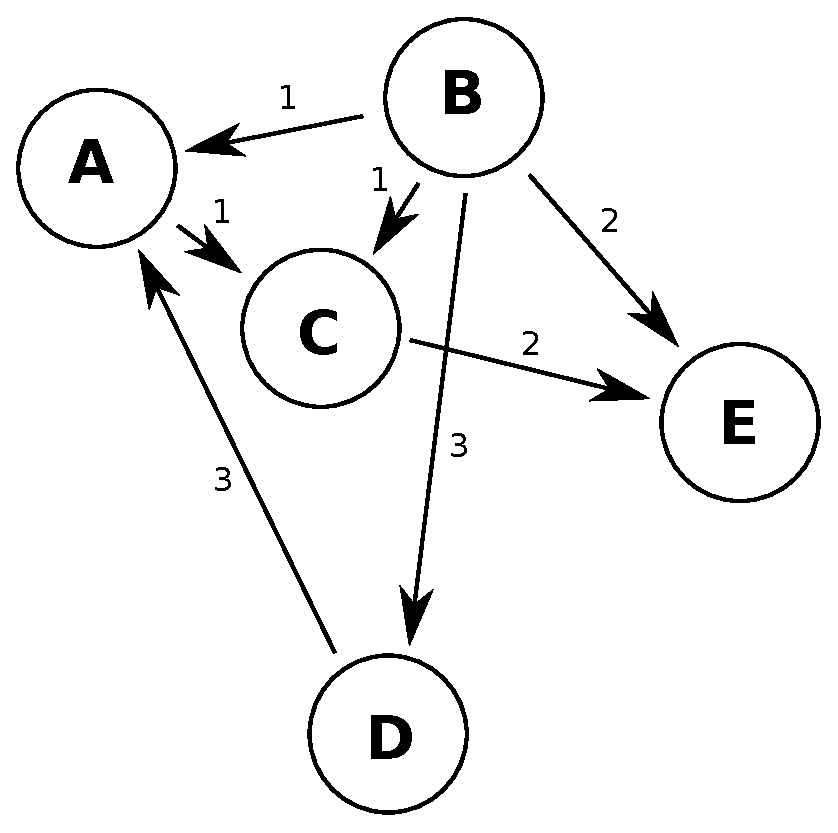
\includegraphics[width=\textwidth]{wNormal.eps}
	\caption{Vážená síť autorů, kde váha odpovídá vzdálenosti mezi uzly}
	\label{fig:wNormal}
\end{minipage}
\hspace{0.5cm}
\begin{minipage}[b]{0.45\textwidth}
\centering
	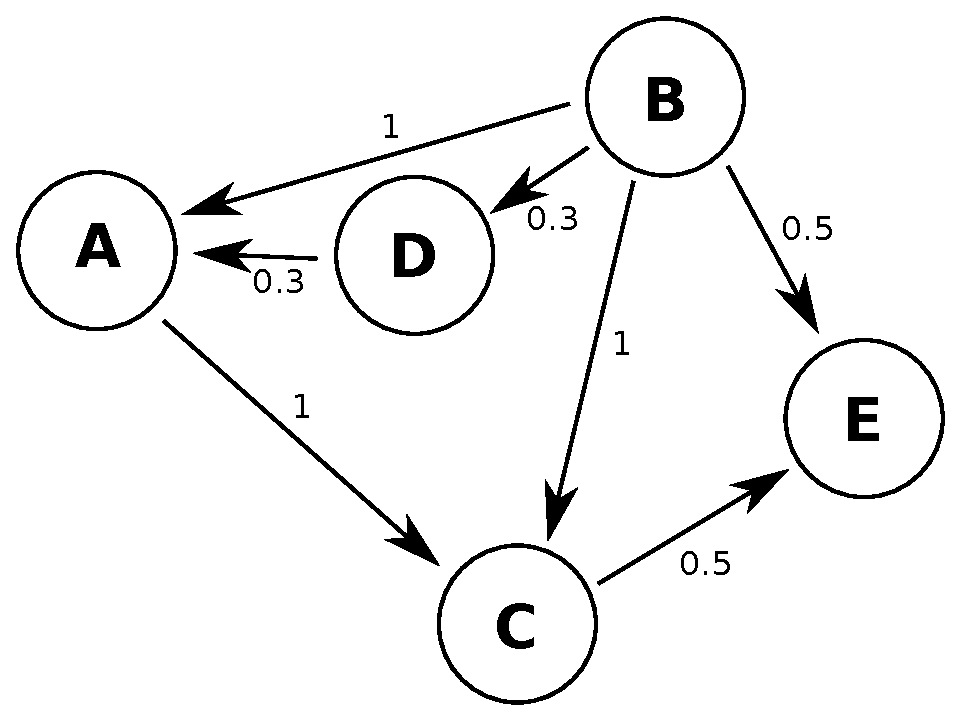
\includegraphics[width=\textwidth]{wRecip.eps}
	\caption{Stejná síť autorů s převrácenou hodnotou váhy ($\frac{1}{w}$)}
	\label{fig:wRecip}
\end{minipage}
\end{figure}

\subsection{Orientované a neorientované sítě}
V případě sociálních sítí nejčastěji uvažujeme sítě bez orientace, protože
nejčastěji modelovaný vztah \uv{přítel-přítel} je ekvivalentní z pohledu obou
koncových uzlů. Pro citační síť jsou na místě orientované hrany, protože vztahy
autor odkazujícího na jiného autora nebo publikace citující jinou publikaci
mají očividně jinou interpretaci z pohledu koncových uzlů. Buďto se jedná o
citovaného nebo citujícího autora či publikaci.


\chapter{Citační databáze}
Bibliografická citační databáze poskytují možnost vyhledávání bibliografických
citací. Velké množství z dnešních citačních databází se zaměřuje na jeden obor.
\citep{libraryamnh}.  Jiné jsou multioborové s možností volby prohledávaného
oboru (Scopus, Web of Science).

\section{DBLP}
DBLP \citep{DBLP} je webová bibliografická databáze hostovaná na univerzitě
Trier. Od 80. let indexovala literaturu z oblasti databázových systémů a
logického programovaní, ale postupně se její zaměření zobecnilo a nyní je
bibliografickou databází obecně pro obor informatiky. 
V roce 2012 obsahovala více než 2,1 milionu článků. Metody implementované v
této práci jsou aplikovány na verzi z roku 2004. 
Tab.~\ref{tab:dblpstat} poskytuje statistiky o vytvořených citačních sítí z
této databáze. Obr.~\ref{fig:dblpweightsdistribution} znázorňuje vlastnosti
bezškálové sítě pro váženou citační síť autorů - čím vyšší váha, tím menší
pravděpodobnost výskytu v síti. Obr.~\ref{fig:dblpdegreedistribution} znázorňuje
mocninné rozdělení stupňů uzlů pro stejnou síť.

\begin{table}[!ht]
\centering
\caption{Statistiky pro databázi DBLP 2004}
\label{tab:dblpstat}
\begin{tabular}{r|l}
\toprule
& hodnota \\
\midrule
Počet publikací & 470\,554 \\
Počet hran v síti publikací & 109\,130 \\
Počet autorů & 315\,485 \\
Počet hran v síti autorů & 331\,245 \\
Počet samocitací & 3\,095 \\
Průměrný počet spoluautorů & 2.278 \\
Největší silně spojitá komponenta & 1.637\% \\
Průměrná nejkratší cesta\footnotemark[1] & 2.894 \\
Průměrná nejkratší cesta\footnotemark[2] & 1.194 \\
Poloměr grafu\footnotemark[1] & 8.0 \\
Poloměr grafu\footnotemark[2] & 6.637 \\
\bottomrule
\end{tabular}
\end{table}
\footnotetext[1]{Platí pro neváženou síť autorů}
\footnotetext[2]{Platí pro váženou síť autorů}

\begin{figure}[!ht]
\centering
	\includegraphics[width=9cm,angle=270]{ewd_dblp.eps}
	\caption{Log-log graf mocninného rozdělení vah hran citační sítě autorů DBLP}
	\label{fig:dblpweightsdistribution}
\end{figure}
\begin{figure}[!ht]
\centering
	\includegraphics[width=9cm,angle=270]{dd_dblp.eps}
	\caption{Log-log graf mocninného rozdělení stupňů uzlů citační sítě autorů DBLP}
	\label{fig:dblpdegreedistribution}
\end{figure}


\section{CiteSeer}
CiteSeer~\citep{citeseer} (nyní CiteSeer$^X$) je považován za první
automatizovaný systém shromažďování publikací a autonomní indexace citací v
nich obsažených. Publikace jsou zejména z oboru informatiky a informační vědy.
V dnešní době obsahuje přes dva miliony dokumentů s téměř dvěma miliony autorů
a čtyřiceti miliony citací. Zde používáme verzi z roku 2005.
Stejně jako u databáze DBLP jsou v tab.~\ref{tab:citeseerstat} uvedeny
statistiky pro vytvořené citační sítě a v
obr.~\ref{fig:citeseerweightsdistribution}
a~\ref{fig:citeseerdegreedistribution} ukázka vlastností bezškálové sítě pro
citační síť autorů.

\begin{table}[!ht]
\centering
\caption{Statistiky pro databázi CiteSeer 2005}
\label{tab:citeseerstat}
\begin{tabular}{r|l}
\toprule
& hodnota \\
\midrule
Počet publikací & 659\,814 \\
Počet hran v síti publikací & 1\,624\,758 \\
Počet autorů & 406\,465 \\
Počet hran v síti autorů & 5\,398\,239 \\
Počet samocitací & 60\,639 \\
Průměrný počet spoluautorů & 2.525 \\
Největší silně spojitá komponenta & 29.763\% \\
Průměrná nejkratší cesta\footnotemark[1] & 4.134 \\
Průměrná nejkratší cesta\footnotemark[2] & 1.592 \\
Poloměr grafu\footnotemark[1] & 15.0   \\
Poloměr grafu\footnotemark[2] & 11.489 \\
\bottomrule
\end{tabular}
\end{table}
\footnotetext[1]{Platí pro neváženou síť autorů}
\footnotetext[2]{Platí pro váženou síť autorů}

\begin{figure}[!ht]
\centering
	\includegraphics[width=9cm,angle=270]{ewd_citeseer.eps}
	\caption{Log-log graf mocninného rozdělení vah hran citační sítě autorů CiteSeer}
	\label{fig:citeseerweightsdistribution}
\end{figure}
\begin{figure}[!ht]
\centering
	\includegraphics[width=9cm,angle=270]{dd_citeseer.eps}
	\caption{Log-log graf mocninného rozdělení stupňů uzlů citační sítě autorů CiteSeer}
	\label{fig:citeseerdegreedistribution}
\end{figure}




\chapter{Analýza sítí}
Více než 40 let byly považovány všechny komplexní sítě za naprosto náhodné.
Paul Erdős a Alfréd Rényi v roce 1959 navrhli modelování komunikačních sítí a
sítí, které se vyskytují v přírodních vědách, spojením uzlů náhodnými hranami.
Tato jednoduchá metoda vytvoření náhodného grafu způsobí rozložení stupňů
vrcholů (počet spojení vrcholu s ostatními) podle Poissonova rozdělení
pravděpodobnosti s charakteristickou křivkou připomínající zvon - většina uzlů
má zhruba stejný stupeň. 
V roce 1998 bylo na univerzitě v Notre Dame (Barabási a kolegové) provedeno
mapování sítě World Wide Web s očekáváním, že výsledkem bude náhodná síť.
Přestože byl zmapován pouze zlomek celé sítě, výsledkem bylo přes všechna
očekávání, zcela jiné rozdělení stupňů - mocninné. Přes $80\%$ uzlů mělo méně
než čtyři spojení, ale méně než $0.01\%$ uzlů mělo více než tisíc spojení.
Sítě, které se řídí mocninným rozdělením stupňů, nazvali Barabási a jeho kolegové
bezškálovými sítěmi (scale-free network). Rozpoznání tohoto jevu vedlo k
lepšímu porozumění šíření virů a epidemií nebo proč některé sítě fungují takřka
beze změny i přes poruchu většiny jejich uzlů.  Sociální a citační sítě se řadí
do kategorie bezškálových sítí. Například autor vědecké literatury, jehož dílo
je v dané oblasti známé, má velkou šanci, že bude citován dalšími autory,
především těmi novými. Stejně tak osoba s velkým počtem přátel má velikou
šanci, že bude představen novým lidem a rozšíří si tak svůj okruh přátel ještě
více. Tomuto jevu v bezškálových sítí se říká \uv{bohatší se stává bohatším}.

Rozvinutou disciplínou v oblasti sítí je analýza sociálních sítí, která se
stala klíčovou technikou v moderní sociologii a stala se významnou v různých
vědeckých oblastech (antropologie, biologie, komunikace, ekonomie, informační
věda, geografie, historie, politologie, ...).

Analýza sociálních sítí zkoumá povahu vztahů (homofilie, multiplexita,
vzájemnost, blízkost vztahů, ...), rozdělení vlastností v síti (míry
centrality, hustota sítě, ...) nebo segmentaci (souvislost grafu, komponenty
grafu, kliky, koeficient shlukování, ...).

\section{Souvislost a komponenty grafu}
Neorientovaný graf je souvislý, pokud pro každé jeho dva vrcholy $u$ a $v$
existuje alespoň jedna cesta z $u$ do $v$. U neorientovaného grafu hovoříme o
slabé souvislosti. Pro orientovaný uvažujeme silnou souvislost, protože
přestože existuje cesta z $u$ do $v$, není zaručeno, že existuje cesta z $v$ do
$u$.  Slabě souvislý orientovaný graf znamená, že neorientovaný graf, který by
vznikl nahrazením orientovaných hran neorientovanými (symetrizace grafu), by
byl souvislý.

Komponenta maximálně souvislý podgraf. Jinak řečeno komponenta je podgraf
takový, že všechny jeho vrcholy jsou spojeny nějakou cestou. Komponentou je i
samostatný vrchol.

Všechny slabě souvislé komponenty grafu najdeme pomocí jednoduchých algoritmů
\uv{prohledávání do šířky} nebo \uv{do hloubky}. Spuštění prohledávání najde
celou komponentu, ve které se výchozí vrchol nachází. Pokud zaznamenáváme,
které vrcholy byly nalezeny, a spustíme prohledávání ze všech nenalezených
vrcholů, najdeme všechny komponenty. 

Silně spojité komponenty nenajdeme pouhým prohledáním do šířky nebo do hloubky,
ale použijeme sofistikovanější algoritmy (Kosarajův, Tarjanův, ...), které
principově vycházejí z prohledávání do hloubky.

\section{Klika v grafu}
Klika (clique) grafu je úplný podgraf. To znamená, že všechny vrcholy kliky
jsou spojeny přímo hranou.

V sociologii slovo klika popisuje skupinu dvou až dvanácti lidí, kteří jsou na
sebe vázáni více než na jiné lidi v tomtéž prostředí~\citep{salkind2008}. Klika
je silněji spojená skupina lidí než sociální kruh.

Algoritmus pro nalezení největší kliky v grafu je přímočaré otestování $n$
vrcholů podgrafu pro všech $2^L$ podgrafů grafu, kde $L$ je horní limit
velikosti podgrafu. Pokud je všech $\frac{n(n - 1)}{2}$ párů vrcholů daného
podgrafu spojených hranou, pak se jedná o kliku. Problém má exponenciální
složitost, proto je horní hranice velikosti podgrafu ve výpočtech omezena na
20.

\section{Významnost uzlů}
Významnost autorů je jedním předmětem zájmu analýzy sociálních sítí. Kdybychom
se měli rozhodnout, kterého člena sítě zvolit jako vůdce nebo přes které členy
nejrychleji rozšíříme zprávu, koho bychom měli vybrat? 

\subsection{Ocenění významných autorů}
Významní autoři vědecké literatury bývají za své dílo oceněni významnou cenou
nebo zařazeni do seznamů významných členů.

Autory, kteří byli oceněni těmito cenami, můžeme považovat za významné a
častokrát citované už jen proto, že přítomností jejich jména v seznamu
oceněných prestižní cenou se dostanou do podvědomí mnoha jiných, zejména
začínajících autorů.

% TODO kecy co to ty ceny jsou a k čemu jsou a proč je tu uvádim.
\subsubsection{ACM A.M. Turing Award}
ACM A.M. Turing Award je ocenění ročně udělované skupinou ACM (Association for
Computing Machinery) jedincům vybraným pro kontribuce technického ducha do
výpočetního světa~\citep{turingaward}.

Turingova cena je brána jako nejvyšší vyznamenání v informatice a je lidově
nazývána Nobelovou cenou pro informatiku \citep[p.~317]{dasgupta}.

\subsubsection{ACM SIGMOD Edgar F. Codd Innovations Award}
ACM SIGMOD Edgar F. Codd Innovations Award je ohodnocení životního díla
skupinou ACM SIGMOD (Special Interest Group on Management of Data) za
inovativní a vysoce ceněné kontribuce k rozvoji, porozumění a použití
databázových systémů a databází \citep{sigmodinnovations}.

\subsubsection{ACM Fellows}
\uv{The ACM Fellows Program} byl založen v roce 1993, aby našel a ocenil
vynikající členy ACM za jejich dílo v informatice a informační vědě a pro
jejich významné kontribuce pro účel ACM. Členové ACM Fellows slouží jako
význační kolegové, ke kterým ACM a jejich členové vzhlížejí jako k autoritám v
době rozvoje informačních technologií \citep{acmfellows}.

\subsubsection{ISI Highly Cited highlighted}
ISI Highly Cited je databáze často citovaných autorů v článcích posledního
desetiletí, které byly publikovány institutem ISI (Institute for Scientific
Information). Ten v dnešní době spadá pod agenturu Thomson Reuters, na jejíchž
webových stránkách nalezneme seznam autorů ISI Highly Cited highlighted z let
2000 až 2008 napříč 21 vědeckými obory \citep{highlycited}.

\section{Míry centrality}
V sítích dopravní infrastruktury nás zajímá, po které cestě se nejrychleji a
nejvýhodněji dostat z bodu $A$ do bodu $B$. V sociálních a citačních sítích
nemůžeme intuitivně hovořit o nějakých cestách mezi uzly, protože ani přesně
nevíme, jak takovou cestu interpretovat. Nejkratší cesta mezi přáteli v
sociální síti může znamenat přes které přátele se mezi nimi nejpravděpodobněji
šíří informace. V sítích spolupráce vědeckých autorů se například setkáme s
tzv. Erdősovým číslem, které vyjadřuje nejkratší vzdálenost mezi osobou a
matematikem Paulem Erdősem v rámci spolupráce na vědeckých článcích v oboru
matematiky.

Použijeme-li metody z dopravních sítí pro analýzu sociálních a citačních sítí,
které v jádře spočívají v hledání nejkratších cest, setkáme se se dvěma
nejznámějšími mírami centrality, a to closeness centrality a betweenness
centrality.

Nechť cesta z bodu $u \in V$ do bodu $v \in V$ je střídající se posloupnost
vrcholů a hran takových, že spojují předcházející a následující vrchol v této
posloupnosti. Délka cesty je pak součet vah hran této cesty nebo pouze počet
hran v případě neváženého grafu. Vzdálenost vrcholů $d_G(u, v)$ je délka
nejkratší z cest, která spojuje vrcholy $u$ a $v$.

Jiné míry jsou založeny na počtu spojení jednoho uzlu s ostatními uzly a
nejkratší cesty neuvažují (degree, eigenvector).


\subsection{Degree}
Stupeň je počet hran spojených s uzlem. Pro orientovaný graf můžeme uvažovat
vstupní (indegree) a výstupní stupeň (outdegree) vrcholu nebo obecný stupeň
(degree), tedy součet těchto dvou. Vstupní stupeň se často označuje jako
$deg^-$ a výstupní jako $deg^+$. Nechť $C_D$ označuje míru centrality degree a
${C_D}_{in}$, ${C_D}_{out}$ centralitry indegree a outdegree, respektive. Pak
můžeme vyjádřit hodnoty centrality pomocí matice sousednosti ${\bf A}$.

\begin{align}
\label{eq:degree}
{C_D}_{in}(u) &= deg^-(u)  = \displaystyle\sum\limits_{v \in V} {\bf A}_{uv} \\
{C_D}_{out}(u) &= deg^+(u) = \displaystyle\sum\limits_{v \in V} {\bf A}_{vu} \\
{C_D}(v) &= {C_D}_{in} + {C_D}_{out}
\end{align}

Pokud uvažujeme pouze vstupní stupeň, vypočtená hodnota určuje významnost uzlu,
kdežto výstupní stupeň ukazuje jakousi společenskost či otevřenost uzlu. 

Degree centrality je výpočetně velmi jednoduchý způsob, jak změřit významnost
prvku v síti. Tato metoda je však příliš jednoduchá, protože do výpočtu hodnoty
centrality nezahrnuje uzly, které jsou od daného uzlu vzdálenější než jeden
krok. Tento fakt je známý problém a důvod pro zavedení dalších a složitějších
metod pro výpočet významnosti.



\subsection{Eigenvector centrality}
Eigenvector centrality (také známá jako Gould's index of accessibility of a
Network~\citep{williams2007} nebo Bonacich's
centrality~\citep{hannemanriddle2005}) je míra vlivu vrcholu v grafu, která
doslova znamená \uv{Důležitý uzel má důležité
sousedy}~\citep{zweigiyengar2010}. Hodnotu vlivu získáme z vlastního vektoru
$x$ matice sousednosti grafu:

\begin{align*}
{\bf Ax} &= \lambda {\bf x}
\end{align*}

${\bf A}$ je matice sousednosti, ${\bf x}$ je vlastní vektor matice ${\bf A}$ a
řešením této rovnice. Rovnice má více řešení. Ke každému řešení náleží vlastní
číslo $\lambda$. Pro měření významnosti nás však zajímá pouze to řešení, které
má pouze nezáporné hodnoty. Podle Perron-Frobeniovy věty pro každou nezápornou
primitivní matici existuje právě jedno takové řešení, které zároveň patří k
největšímu vlastnímu číslu $\lambda$~\citep{langvillemeyer}.

Rovnici můžeme rozepsat z maticového tvaru do jednotlivých složek:

\begin{align*} 
x_u &=  \frac{1}{\lambda} \displaystyle\sum_{v \in V} {\bf A}_{uv} x_v 
\end{align*} 

Kde $x_u$ je prvek vlastního vektoru ${\bf x}$
náležící vrcholu $u$ a ${\bf A}_{uv}$ je prvek matice sousednosti ${\bf A}$,
který leží na řádku $u$ a sloupci $v$.

\begin{align*} 
{x_u}_{i + 1} &=  \frac{1}{\lambda} \displaystyle\sum_{v \in V} {\bf A}_{uv}
{x_v}_{i}
\end{align*} 

V tomto rekurentním tvaru je vidět předpis pro iterační výpočet eigenvector
centrality. Algoritmus se nazývá mocninná metoda, která se používá pro řešení
problému vlastních čísel v numerické matematice. Výsledkem mocinné metody je
dominantní vlastní číslo a odpovídající vlastní vektor. Pro eigenvector
centrality nás zajímá právě tohle řešení a žádné jiné.

Z druhé rovnice si navíc povšimneme, že se jedná o přímé rozšíření degree
centrality~\eqref{eq:degree}. Výsledek předchozí iterace použijeme jako vstup
do následující a iterujeme tak dlouho, dokud nedosáhneme požadované přesnosti.

\subsubsection{PageRank}
V roce 1998 vyvinuli Sergey Brin a Larry Page algoritmus PageRank (nesoucí
jméno druhého autora) jako součást výzkumu na novém druhu webového
vyhledávače~\citep{pagerankoriginal,visemalseed2005,page1997}. PageRank
přiřazuje relativní hodnocení webovým stránkám podle hypertextových odkazů z
jiných webových stránek, které na ně směřují, a podle jejich PageRankové
významnosti. Sama definice je rekurzivní a po nahlédnutí na vzorec zjistíme, že
se jedná o rozšířenou variantu algoritmu pro eigenvector centrality.

\begin{align*}
{x_u}_{i + 1} &= \frac{1 - d}{|V|} + d \displaystyle\sum_{v \in V} {\bf A}_{uv}
\frac{{x_v}_{i}}{deg^+ (v)}
\end{align*}

${\bf A}$ je opět matice sousednosti, $V$ je množina vrcholů a $deg^+(v)$ je
výstupní stupeň vrcholu $v$.  V původní myšlence, kdy PageRank modeluje chování
náhodného surfaře, damping factor $d$ je pravděpodobnost, že daný surfař
přestane opakovaně klikat na odkazy, které najde na webové stránce, na kterou
se dostal z předchozího odkazu, a otevře zcela novou stránku, ze které povede
podobný sled surfování přes odkazy.  Damping factor bývá ze zkušenosti
nastavován na $85\%$.

Hodnota PageRanku je z matematického hlediska pravděpodobnost, že surfař, který
náhodně kliká na odkazy, se dostane na konkrétní stránku. Součet hodnot
PageRanku všech uzlů v síti je tedy $1$, protože PageRank je rozdělení
pravděpodobnosti.

Jedním problémem algoritmu PageRank jsou \uv{visící uzly} (dangling nodes), tj.
uzly bez výstupních hran. Protože musíme v každé iteraci algoritmu zachovat
vlastnost rozdělení pravděpodobnosti, tj. suma všech pravděpodobností je $1$,
je třeba zajistit, aby se přenášená hodnota mezi iteracemi neztrácela právě v
uzlech bez výstupních hran. Problém lze řešit tak, že se tyto uzly z výpočtu
vynechají, nebo přidáním zpětných odkazů z těchto uzlů zpět do sítě.  V každé
iteraci předem vypočítáme součet hodnot PageRanku, které by se ztratily v
uzlech bez výstupních hran ($D$). Tahle hodnota je v rámci iterace konstantní a
pouze ji rovnoměrně rozdělíme mezi uzly sítě (s váhou $1/|V|$).

\begin{align*}
{x_u}_{i + 1} &= \frac{1 - d}{|V|} + d \displaystyle\sum_{v \in V} {\bf A}_{uv} \frac{{x_v}_i}{deg^+ (v)} + \frac{1}{|V|} \displaystyle\sum_{w \in D} {x_w}_i
\end{align*}


\begin{center}
\begin{minipage}{\textwidth}
\begin{algorithm}[H]
	\caption{PageRank}
		\label{alg:pagerank}

	\begin{algorithmic}[1]
	\Statex
	\State $x_0[v] \gets \frac{1}{|V|}$, $v \in V$\Comment{Uzly začínají se stejnou pravděpodobností}
	\For{$i \gets 0, K$}\Comment{Iterujeme $K$-krát, dokud není dosažena požadovaná přesnost}
		\State $s \gets 0$\Comment{$s$ je suma PageRanků pro dangling nodes}
		\For{$v \in V$}
			\If{$deg^+(v) = 0$}
				\State $s \gets s + x_{i}[v]$
			\EndIf
		\EndFor
		\State $x_{i + 1}[v] \gets \frac{s}{|V|}$, $v \in V$\Comment{Každý uzel začíná s přebytkem z dangling nodes}
		\For{$v \in V$}
			\For{$k \in inLinks[v]$}
				\State $x_{i + 1}[v] \gets x_{i + 1} + \frac{x_i[k]}{deg^+(k)}$
			\EndFor
		\EndFor
		\State $x_{i + 1}[v] \gets \frac{1 - d}{|V|} + d x_{i + 1}[v]$, $v \in V$\Comment{Přidání damping factoru}
	\EndFor
	\end{algorithmic}
\end{algorithm}
\end{minipage}
\end{center}
\mbox{}

Přestože je PageRank původně určený pro webovou síť, lze ho použít na
jakoukoliv orientovanou váženou i neváženou síť, tedy i na sociální a citační
sítě, o kterých je zde řeč. Pro neorientovaný graf je hodnota PageRanku pro
jednotlivé uzly velmi blízká stupňům grafu, ale ne
totožná~\citep{perrafortunato2008}.


\subsection{Closeness centrality}
Closeness neboli \uv{blízkost} je definována jako převrácená hodnota míry
farness, tedy \uv{dalekost}~\citep{sabidussi1966}. Dalekost je součet všech
vzdáleností od uzlu do všech ostatních, tzn. $f(u) = \sum_{v \in V} d_G(u, v)$
a $c(u) = \sum_{v \in V} \frac{1}{d_G(u, v)}$. Podle jiné definice je closeness
převrácená hodnota průměrné nejkratší cesty. V podstatě se od předchozí příliš
neliší, protože průměrná nejkratší cesta je rovna $\frac{1}{|V|
- 1} \sum_{v \in V} d_G(u, v)$ a closeness podle této definice:

\begin{align*}
c(u) &= \frac{|V| - 1}{\sum_{v \in V} d_G(u, v)}
\end{align*}

Pro obě definice platí, že čím vyšší hodnota $c(u)$, tím je uzel $u$
významnější podle této míry. Zde se budeme soustředit na druhou definici,
protože je častou volbou autorů zabývajících se touto problematikou a existuje
pro ni aproximační algoritmus, který si zde uvedeme.

Closeness, stejně jako ostatní míry centrality, modeluje rozptýlení informace
napříč sítí. Výše uvedené klasické definici je vytýkáno, že pro přenos
informace uvažuje pouze nejkratší cesty, které nejsou vždy jedinou komunikační
cestou v síti. Alternativu navrhli Noh a Rieger (2004), kde namísto nejkratších
cest používají náhodné procházky (random walk closeness centrality). Náhodná
procházka (random walk) je cesta, kde v každém uzlu je náhodně vybrán směr
dalšího postupu.

Příkladem může být oběh mincí mezi lidmi. Tento jev nemá s nejkratšími cestami
mnoho společného, proto je vhodnější ho modelovat náhodnými procházkami. Oproti
tomu například poštovní zásilky očividně cestují po nejkratších cestách. Pokud
uvažujeme citační sítě, nemáme jasnou představu o významu náhodných procházek
nebo nejkratších cest jako v případě mince nebo dopisu. I přesto očekáváme
vysokou podobnost této metody s ostatními.

Nevýhodou closeness centrality je nutnost uvažovat souvislý graf, tedy takový,
který obsahuje pouze jednu komponentu. Pokud by měl více komponent, pak by vždy
existovala cesta s nekonečnou vzdáleností. Hodnota farness by pak byla
automaticky nekonečná a closeness, tedy převrácená hodnota, by byla nulová. 

Existuje několik upravených definic, které se mají vypořádat s problémem
konektivity a druhotně jsou numericky stabilnější. Jedna z nich zaměňuje
převrácenou hodnotu součtu vzdáleností za součet převrácených hodnot
vzdáleností $c(u) = \sum_{v \in V} \frac{1}{d_G(u, v)}$ (Opsahl) a druhá $c(u)
= \sum_{v \in V} 2^{-d_G(u, v)}$ (Dangalchev). Přesto se nejvíce používá
původní definice closeness a výpočet se omezí na největší komponentu.


\subsubsection{Algoritmus}
Closeness pro všechny vrcholy můžeme přesně vypočítat v čase $O(|E| +
|V|^2\log|V|)$, kde $V$ a $E$ jsou množiny vrcholů a hran
sítě~\citep{fredmantarjan}.

Algoritmus vychází z definice, tedy vyřeší problém všech párů nejkratších cest,
čímž rovnou získá hodnoty farness $f(u) = \sum_{v \in V} d_G(u, v)$ a zjištění
closeness je poté triviální podle jedné z výše uvedených definic.  Výše uvedená
složitost platí při použití Dijkstrova algoritmu pro všechny páry cest.

\begin{center}
\begin{minipage}{\textwidth}
\begin{algorithm}[H]
	\caption{Closeness}
		\label{alg:closeness}

	\begin{algorithmic}[1]
	\Statex
	\For{$s \in V$}
		\State $f \gets 0$\Comment{Farness}
		\State $d[v] \gets \infty$, $v \in V$\Comment{Zpočátku jsou uzly nedosažitelné}
		\State $d[u] \gets 0$
		\State $Q \gets \{s\}$\Comment{Prioritní fronta $Q$ začíná se zdrojovým vrcholem}
		\While{$Q \ne \varnothing$}\Comment{Dokud není fronta prázdná}
			\State $u \gets extract\mbox{-}min(Q)$\Comment{Vytáhneme uzel s min. vzdáleností $d$}
			\State $f \gets f + d[u]$\Comment{Zvýšíme farness pro nový uzel}
			\For{sousedící vrchol $v \in Adj[u]$}\Comment{Přidáme nově nalezené vrcholy}
				\If{$d[v] > d[u] + w(u, v)$}
					\State $d[v] \gets d[u] + w(u, v)$
					\State $Q \gets Q \cup \{v\}$
				\EndIf
			\EndFor
		\EndWhile
		\State $c[s] \gets \frac{n - 1}{f}$\Comment{Closeness je převrácená hodnota farness}
	\EndFor
	\end{algorithmic}
\end{algorithm}
\end{minipage}
\end{center}
\mbox{}

Výpočet closeness lze snadno paralelizovat, jelikož výpočet stromu nejkratších
cest je nezávislá úloha pro každý z $|V|$ vrcholů.

Pro rozsáhlé sítě s miliony uzlů (sociální sítě k dnešnímu datu) je tato metoda
příliš náročná. Eppstein a Wang vyvinuli aproximační algoritmus s náročností
$O(\frac{\log|V|}{\epsilon}^2 (|V| \log |V| + |E|))$ s chybou $\epsilon \delta$
pro převrácenou hodnotu closeness (s pravděpodobností alespoň $1 -
\frac{1}{|V|}$), kde $\epsilon > 0$ a $\delta$ je poloměr sítě (nejdelší z
nejkratších cest). Na základě tohoto aproximačního algoritmu byl vytvořen jiný
aproximační algoritmus pro nalezení $k$ nejvýznamnějších uzlů hodnocených podle
closeness centrality TOPRANK~\citep{closenessapproximation}.

\subsubsection{Aproximace}
Algoritmus TOPRANK najde prvních $k$ nejvýznamnějších uzlů
s vysokou přesností a pro každý z nich přesnou hodnotu closeness.  Algoritmus
pracuje s myšlenkou, že zjistíme přibližné pořadí uzlů tak, že pro jeden strom
nejkratších cest nebudeme počítat se všemi koncovými uzly, ale jen s dostatečně
velkým vzorkem této množiny.  Přesné hodnoty closeness dosáhneme použitím
exaktního algoritmu, který použijeme jen na nejvýznamnější uzly získané z
prvního aproximovaného kroku. Klíčovou otázkou je, kolik nejvýznamnějších uzlů
musíme uvažovat, aby se jednalo o dostatečně přesný výsledek. Autoři algoritmu
uvádějí tento algoritmus s heuristikou, která najde přibližně místo, ve kterém
je vhodné výpočet ukončit a považovat za dostatečně přesný. Sami uvádějí, že
tento algoritmus je pouze první krok k návrhu efektivnějšího způsobu jak najít
prvních $k$ nejvýznamnějších uzlů~\citep{closenessapproximation}.

\subsection{Betweenness centrality}
Betweenness je druhá metoda, která modeluje šíření informace sítí pomocí
nejkratších cest. Princip betweenness spočívá ve zvýhodnění uzlů, přes kterou
teče nejvíce informace. Pokud uzel $A$ komunikuje s uzlem $C$, můžeme tvrdit,
že uzel $B$, který leží mezi nimi, bude mít roli prostředníka. Být tímto
prostředníkem mezi více uzly intuitivně napovídá, že takový uzel bude
centrální. \uv{Čím více lidí na mně závisí k vytvoření spojení s jinými lidmi,
tím mám větší moc}~\citep{hannemanriddle2005}. Betweenness
měří, na kolika nejkratších cestách se uzel nachází. Více se ale setkáme s
definicí, kde do sumy zahrneme poměr cest, na kterých se uzel nachází, k
celkovému počtu cest mezi dvěma uzly~\citep{freeman1977,anthonisse1971,brandes2001}.

\begin{align*}
C_(v) &= \displaystyle\sum\limits_{s \in V} \displaystyle\sum\limits_{t \in V \backslash s} \frac{\sigma_{st}(v)}{\sigma_{st}} \\
\end{align*}

$C_b(v)$ značí hodnotu betweenness centrality pro uzel $v$, V množinu všech
uzlů grafu, $\sigma_{st}$ je počet nejkratších cest mezi uzly $s$ a $t$ a
$\sigma_{st}(v)$ je počet nejkratších cest, které navíc procházejí uzlem $v$.

Normalizovaný betweenness je hodnota v intervalu od $0$ do $1$, kterou získáme
tak, že betweenness vydělíme celkovým počtem možných cest, tj. $(|V| - 1)(|V| -
2)$ pro orientované grafy a $\frac{(|V| - 1)(|V| - 2)}{2}$ pro neorientované
grafy. Normalizované hodnoty metod centralit jsou nezávislé na velikosti
grafu~\citep{whiteborgatti1994}.

\begin{align*}
C_b(v) &= \frac{1}{(|V| - 1)(|V| - 2)} \displaystyle\sum\limits_{s \in V} \displaystyle\sum\limits_{t \in V \backslash s} \frac{\sigma_{st}(v)}{\sigma_{st}} \\
\end{align*}

Vznik betweenness je připisován sociologovi Lintonu
Freemanovi~\citep{freeman1977} a byl původně definován pro neorientované grafy.

\subsubsection{Brandesův algoritmus}
Ve své práci~\citep{brandes2001} Ulrik Brandes zmiňuje (do té doby
nejrychlejší) algoritmus pro výpočet betweenness centrality s časovou
náročností $\theta(|V|^3)$ a $\theta(|V|^2)$ paměťovými nároky. Tento způsob
přistupuje k problému nekratších cest způsobem all-pair shortest paths.
Brandesův způsob využívá algoritmu pro nalezení nejkratších cest z jednoho
bodu, kde výsledný algoritmus pracuje s paměťovou náročností $O(|V| + |E|)$ a
běží v čase $O(|V||E|)$ pro nevážený graf nebo $O(|V||E| + |V|^2 \log|V|)$ pro
vážený graf. 

%% TODO napsat pár větama brandes alg., aby se dala pochopit aproximace.

Brandes ve své práci o algoritmu uvádí pseudokód pro nevážený graf, který je
následně snadné pozměnit pro vážený graf drobnými úpravami a zaměněním obyčejné
fronty za prioritní frontu; kompletní důkaz správnosti algoritmu a porovnání
standardního algoritmu s tímto~\citep{brandes2001}.



\begin{center}
\begin{minipage}{\textwidth}
\begin{algorithm}[H]
	\caption{Brandes}
		\label{alg:brandes}

	\begin{algorithmic}[1]
	\Statex
	\State $b[v] \gets 0$, $v \in V$\Comment{Inicializujeme hodnoty betweenness na 0}
	\For{$s \in V$}\Comment{V exaktním výpočtu počítáme s celou množinou V}
		\State $S \gets $prázdný zásobník\Comment{Zásobník pro \uv{dokončené} vrcholy}
		\State $P[w] \gets $prázdný seznam, $w \in V$\Comment{Seznam předchůdců}
		\State $\sigma[t] \gets 0$, $t \in V$
		\State $\sigma[s] \gets 1$
		\State $d[t] \gets -1$, $t \in V$\Comment{Vzdálenosti jsou inicializovány na -1, tj. symbolicky nekonečno}
		\State $d[s] \gets 0$
		\State $Q \gets \{s\}$\Comment{Fronta nebo prioritní fronta začíná se startovním vrcholem}
		\While{$Q \ne \varnothing$}\Comment{Opakujeme, dokud není fronta prázdná}
			\State $v \gets dequeue(Q)$
			\State $push(S, v)$
			\For{sousedící vrchol $w \in Adj[v]$}
				\If{$d[w] < 0$}
					\State $enqueue(Q, w)$
					\State $d[w] \gets d[v] + 1$
				\EndIf
				\If{$d[w] = d[v] + 1$}\Comment{Nejkratší cesta do $w$ přes $v$?}
					\State $\sigma[w] \gets \sigma[w] + \sigma[v]$
					\State $push(P[w], v)$
				\EndIf
			\EndFor
		\EndWhile
		\State $\delta[v] \gets 0$,$v \in V$\Comment{$\delta$ je závislost uzlu $s$ na ostatních}
		\While{$S \ne \varnothing$} \Comment{$S$ vrátí vrcholy v pořadí s nezvyšující se vzdáleností od $s$}
			\State $w \gets pop(S)$
			\For{$v \in P[w]$}
				\State $\delta[v] \gets \delta[v] + \frac{\sigma[v]}{\sigma[w]}(1 + \delta[w])$
			\EndFor
			\If{$w \ne s$}\Comment{Betweenness je součet dependencí $\delta[w]$}
				\State $b[w] \gets b[w] + \delta[w]$
			\EndIf
		\EndWhile
	\EndFor
	\end{algorithmic}
\end{algorithm}
\end{minipage}
\end{center}
\mbox{}


% Závislost (dependency) vrcholu $s \in V$ na všech ostatních vrcholech je v
% tomto algoritmu (cite Brandes):
% \begin{align*}
% \delta_{s \bullet}(v) &= \displaystyle\sum\limits_{w:v \in P_s(w)} \frac{\sigma_{sv}}{\sigma_{sw}}(1 + \sigma_{s \bullet}(w))
% \end{align*}

Algoritmus lze paralelizovat stejně jako algoritmus pro closeness centrality,
pokud zajistíme synchronizaci vláken při přístupu k hodnotám betweenness.
Narozdíl od algoritmu pro closeness, kde výpočet pro jeden uzel ovlivňuje
hodnotu closeness pouze pro tento uzel, u betweenness výpočet vycházející z
jednoho uzlu ovlivňuje hodnotu betweenness potencionálně i pro všechny ostatní
uzly.

\subsubsection{Aproximace}
I přes použití rychlejšího Brandesova algoritmu je výpočet betweenness
centrality příliš náročný výpočet pro sítě reálného světa (např. biologické,
dopravní nebo webové sítě) a pokud nám jde více o relativní pořadí uzlů podle
hodnoty betweenness než o hodnotu samotnou, lze oželit přesný výpočet
přibližným, který příliš nezmění výsledné umístění v žebříčku nejvýznamnějších
uzlů.

Bader, Kintali, Madduri, Mihail ukazují aproximační algoritmus pro betweenness
s odhadem chyby.  Myšlenkou je jednoduchá lineární extrapolace Brandesova
algoritmu, pokud do výpočtu zahrneme pouze náhodný vzorek namísto celé množiny
vrcholů. Nechť $k$ je velikost vzorku množiny vrcholů, se kterým počítáme, pak
extrapolovaná hodnota betweenness je $\frac{|V| S}{k}$, kde $S$ je vypočtená
přibližná hodnota.


\section{Hledání nejkratších cest}
Hledání nejkratších cest v grafu je historicky starý problém, jehož matematický
výzkum přišel relativně pozdě v porovnání s jinými problémy kombinatorické
optimalizace (nejmenší kostra grafu, přiřazovací a dopravní problém).
Pravděpodobně byl výzkum opožděn, protože se jedná o intuitivní a relativně
jednoduchý problém, ale jakmile se dostal do středu zájmu, bylo nezávisle na
sobě nalezeno několik metod řešení různými lidmi (Shimbel~\citep{shimbel1955}, Ford~\citep{ford1956}, Dantzig~\citep{dantzig1957}, Bellman~\citep{bellmanford_algorithm}, Moore~\citep{moore1959}, Dijkstra~\citep{dijkstra1959})~\citep{schrijver2012}.


Z hlediska metod řešení můžeme uvažovat několik kategorií algoritmů - nalezení
všech párů nejkratších cest (all-pairs shortest paths problem), nalezení
nejkratší cesty mezi počátečním a koncovým vrcholem (source-target) nebo
nalezení stromu nejkratších cest, máme-li zadán počáteční vrchol (single source
shortest path problem).


\subsection{Single source shortest path}
Pokud hledáme pouze jednu cestu mezi dvěma vrcholy (source-target), nemusíme
počítat celý strom nejkratších cest, ale můžeme zastavit výpočet při dosažení
požadovaného vrcholu. 

\subsubsection{BFS}
Prohledávání do šířky z jednoho bodu (breadth first search) je algoritmus,
který najde nejkratší cesty z jednoho bodu do všech ostatních v případě
neváženého grafu v čase $O(E)$. Pro vážený graf by zjistil nejkratší cesty, kde
metrika vzálenosti by byla počet skoků mezi uzly.

\begin{center}
\begin{minipage}{\textwidth}
\begin{algorithm}[H]
	\caption{Prohledávání do šířky}
		\label{alg:bfs}
	\begin{algorithmic}[1]
	\Statex
	\Function{BFS}{$G, s$}
		\State $d[v] \gets \infty$,$v \in V$\Comment{Uzly jsou zpočátku nedosažitelné}
		\State $d[s] \gets 0$
		\State $p[v] \gets $ NIL,$v \in V$\Comment{A nemají implicitně žádné předchůdce}
		\State $Q \gets \{s\}$\Comment{Fronta začíná s počátečním vrcholem}
		\While{$Q \ne \varnothing$}\Comment{Dokud není prázdná}
			\State $u \gets dequeue(Q)$
			\For{sousedící vrchol $v \in Adj[u]$}
				\If{$d[v] = -1$}\Comment{Pro všechny nově objevené vrcholy}
					\State $d[v] \gets d[u] + 1$\Comment{Nově vypočtená vzdálensot}
					\State $Q \gets Q \cup \{v\}$\Comment{Přidáme nově objevené uzly do fronty}
					\State $p[v] \gets u$\Comment{Předchůdce uzlu $v$ je $u$}
				\EndIf
			\EndFor
		\EndWhile
		\State \textbf{return} $p$
	\EndFunction
	\end{algorithmic}
\end{algorithm}
\end{minipage}
\end{center}
\mbox{}

\subsubsection{Bellman-Fordův algoritmus}
Bellman-Fordův algoritmus je aplikací dynamického programování na nejkratší
cesty z jednoho vrcholu do všech ostatních. Jeho využití najdeme zejména tam,
kde se mohou objevit záporné váhy hran. Časová náročnost je $O(|V||E|)$.

\subsubsection{Dijkstrův algoritmus}
Dijkstrův algoritmus řeší \uv{single source shortest path problém} pomocí greedy
(žravé) strategie. Časová náročnost běžné implementace $O((|E| + |V|)\log|V|)$
je lepší než u Bellman-Fordova algoritmu, ale Dijkstrova greedy strategie
funguje, pouze pokud v grafu neexistují záporně ohodnocené hrany. Časová
náročnost závisí především na implementaci klíčové datové struktury prioritní
fronty, která v každém kroku vybírá uzel s nejmenší vzdáleností od zdrojového
vrcholu (greedy strategie). V případě použití obyčejného spojového seznamu jako
prioritní fronty získáme kvadratickou náročnost $O(|V|^2)$. Nejčastěji se
setkáme s prioritní frontou implementovanou pomocí binární haldy, která
zajišťuje čas běhu právě $O((|E| + |V|)\log|V|)$. Pomocí Fibonacciho haldy
získáme doposud nejrychlejší Dijkstrův algoritmus s časem běhu $O(|E| + |V|
\log|V|)$, ale pro běžné účely (grafy menší než miliony vrcholů) je
nejvýhodnější binární halda~\citep{CLRS,fredmantarjan}. Pro nevážený graf
je Dijkstrův algoritmus ekvivalentní prohledávání do šířky.

Dijkstrův algoritmus je klíčovým pro všechny implementované metody založené na
nejkratších cestách, proto uvedeme pseudokód~\citep{CLRS}.

\begin{center}
\begin{minipage}{\textwidth}
\begin{algorithm}[H]
	\caption{Dijkstrův algoritmus}
		\label{alg:dijkstra}
	\begin{algorithmic}[1]
	\Statex
	\Function{Dijkstra}{$G, w, s$}  \Comment{$s$ je zdrojový vrchol a $w$ je váhová funkce}
		\State $d[v] \gets \infty$,$v \in V$\Comment{Vrcholy jsou zpočátku nedosažitelné}
		\State $d[s] \gets 0$
		\State $p[v] \gets $ NIL,$v \in V$\Comment{Předchůdci vrcholů zpočátku neexistují}
		\State $Q \gets V$\Comment{Prioritní fronta $Q$ obsahuje všechny vrcholy}
		\While{$Q \ne \varnothing$}\Comment{Postupujeme, dokud není prázdná}
			\State $u \gets extract\mbox{-}min(Q)$\Comment{Vytáhneme z fronty vrchol s nejmenší hodnotou $d[u]$}
			\For{sousedící vrchol $v \in Adj[u]$}
				\If{$d[v] > d[u] + w(u, v)$}
					\State $d[v] \gets d[u] + w(u, v)$\Comment{Relaxace hrany $\{u, v\}$}
					\State $p[v] \gets u$
				\EndIf
			\EndFor
		\EndWhile
		\State \textbf{return} $p$\Comment{Strom předchůdců}
	\EndFunction
	\end{algorithmic}
\end{algorithm}
\end{minipage}
\end{center}
\mbox{}

Výsledkem je strom předchůdců, který reprezentuje strom nejkratších cest.
Princip Dijkstrova algoritmu se objevuje i u algoritmů pro closeness,
betweenness a BFS. V tomto případě do prioritní fronty prvotně zahrneme všechny
vrcholy. Jinou možností je přidávat je postupně, aby vybírání z prioritní
fronty ($extract\mbox{-}min(Q)$) bylo rychlejší. Tento způsob je použit v
algoritmu pro closeness.
% TODO reference algs

%\subsubsection{Orientovaný acyklický graf}
%Pro orientovaný acyklický graf (directed acyclic graph), kterým je například
%citační síť publikací, neboť není možné, aby publikace referencovala publikaci
%do budoucna, je vhodné využít vlastnost absence cyklů. Algoritmus pro nalezení
%nejkratších cest z jednoho bodu do všech ostatních pro orientovaný acyklické
%graf využívá topologického seřazení a principu dynamického programování:

\subsection{All-pair shortest paths}
Do této kategorie spadají maticové metody, tj. graf je zadán jako matice
sousednosti nebo matice sousednost s váhami hran.


\subsubsection{Shimbelova metoda}
Shimbelova metoda (1955) používá upravené maticové násobení k získání $|V|$-té
mocniny matice sousednosti. Celková časová náročnost je $O(|V|^4)$, protože
provedeme $|V|$ \uv{násobení} čtvercové matice o složitosti $O(|V|^3)$.
Shimbelovo upravené násobení nahrazuje sčítání a násobení za minimum a sčítání:

\begin{align*}
x + y &\equiv \min(x, y) \\
xy &\equiv x + y
\end{align*}

\subsubsection{Floyd-Warshallův algoritmus}
Floyd-Warshallův algoritmus snižuje časovou náročnost na $O(|V|^3)$
použitím dynamického programování. Graf je opět zadán jako vážená matice
sousednosti. Rekurentní vzorec dynamického programování pro tento algoritmus je:

\begin{align*}
d_0(u, v) &= {\bf A}_{uv} \\
d_{k + 1}(u, v) &= \min(d_k(u, v), d_k(u, k) + d_k(k, v)) \\
\end{align*}

Jednodušše zkoušíme, zda je kratší cesta mezi vrcholy $u$ a $v$, kterou již
známe, nebo jiná cesta za použití nějakého vrcholu $k$, který leží mezi nimi.
Výpočet provádíme pro všechny páry vrcholů pro každý vrchol $k$ ($|V|^2 |V|$).

\subsubsection{Johnsonův algoritmus}
Johnsonův algoritmus nepatří mezi maticové metody, protože využívá
metod single source shortest path pro všechny vrcholy. V principu jednodušše
použijeme Dijkstrův algoritmus pro každý vrchol zvlášť, ale dovolujeme váhy
hran i záporné. V případě záporných hran je nutné provést transformaci vah
pomocí Bellman-Fordova algoritmu, která v grafu nepozmění nejkratší cesty~\citep{CLRS}.


\section{Ostatní míry významnosti autorů}
Míry centrality jsou určeny pro relativní seřazení uzlů pro obecný graf.
Jelikož zde pracujeme speciálně s citačními sítěmi, zajímá nás, jestli existují
i jiné metody ohodnocení autorů, které ani nevyžadují konstrukci citačních
sítí, ale vyžadují pouze údaje v databázi.

Setkáme se s metodami AWCR, AW-index, Eigenfactor, Egghův g-index, E-index,
I10-index, R-impact, Wu Index a zejména H-index~\citep{hlwikiaim}, který zde
byl implementován jako jediná metoda, která nespadá pod míry centrality.

\subsection{H-index}
H-index je metoda pro měření produktivity autora a významu jeho publikované
vědecké práce. Metoda byla navržena fyzikem Jorge E. Hirschem pro zjištování
relativní významnosti vědců publikujících v oboru teoretické fyziky. Původní
Hirschova definice zní:

\begin{quote}\textit{
Vědec má index $h$ pokud $h$ z jeho $N_p$ publikací má každá alespoň $h$ citací
a žádná ze zbylých ($N_p - h$) publikací nemá více než $h$ citací.
}
\end{quote}

Tato metoda je specifická pro citační sítě a nelze ji aplikovat na sociální
nebo obecnou komplexní síť.

Výpočet probíhá tak, že seřadíme autorovy publikace $P$ sestupně podle počtu
citací $c: P \mapsto \mathbb{N}$ a poté od začátku tohoto seřazeného seznamu
hledáme tu publikaci, jejíž pořadové číslo v tomto seznamu je nižší nebo rovné
počtu jejích citací. Toto číslo je pak h-index autora.
\begin{center}
\begin{minipage}{\textwidth}
\begin{algorithm}[H]
	\caption{H-index}
		\label{alg:hindex}

	\begin{algorithmic}[1]
	\Statex
	\Function{H-index}{$P, c$}
		\State $sort(P, key \gets c)$\Comment{Seřadíme publikace sestupně podle počtu citací}
		\State $h \gets 1$
		\For{$p \in P$}
			\If{$c(p) \leq h$}\Comment{Bod, kde počet citací vyrovná $h$, je h-index autora}
				\State \textbf{break}
			\EndIf
			\State $h \gets h + 1$
		\EndFor
		\State \textbf{return} $h$
	\EndFunction
	\end{algorithmic}
\end{algorithm}
\end{minipage}
\end{center}
\mbox{}



% \section{Reprezentace citační sítě}

% \subsection{Paralelní výpočty}


% \subsubsection{Charakteristika}


\chapter{Výsledky}
Výsledky této práce jsou znázorněny v tabulkách korelací mezi jednotlivými
metodami (tab.~\ref{tab:corr1}, \ref{tab:corr2}, \ref{tab:corr3}, \ref{tab:corr4}), tabulkami (tab. ) srovnávající pořadí prvních
třiceti autorů mezi jednotlivými metodami a porovnání implementovaných metod s
oceněními (ACM Codd, ...)


\section{Porovnání implementovaných metod}
Zajímá nás, zda-li jsou metody mezi sebou podobné a do jaké míry. Pro porovnání
metod mezi sebou je použit Spearmanův koeficient pořadové korelace.


Tab.~\ref{tab:corr1} ukazuje vypočtené Spearmanovy koeficienty pořadové
korelace mezi všemi páry implementovaných metod. Do výpočtu koeficientu
korelace byly zahrnuty pouze ty uzly, které mají alespoň jednu hranu. Pokud by
byly zachovány, většina koeficientů korelace by byla velmi vysoká (větší než
$0.95$), protože většina vrcholů, zejména v databázi DBLP, jsou osamocené
vrcholy. Protože jsou výsledky seřazeny podle hodnoty centrality a poté podle
jména autora, všechny tyto izolované vrcholy, které nijak nepřispívají k
hodnotě centrality, jsou pro všechny metody umístěné na posledních pozicích v
tomtéž pořadí. Důsledkem je vysoký koeficient korelace, který nám však nic
nevypoví o podobnosti výsledků metod.

Jelikož výpočet pro centralitu closeness ve všech implementovaných variantách
(vstupní hrany, výstupní hrany, vážený closeness) byl proveden pouze na
největší silně spojité komponentě, nelze přímo provést srovnání pomocí
koeficientu korelace s výsledky metod, které byly aplikovány na celý graf,
protože se jedná o dvě neporovnatelné proměnné. Proto byli z výsledků metod pro
celý graf odebráni ti autoři, kteří se nenacházejí v hlavní silně spojité
komponentě. Pro tyto žebříčky bylo provedeno stejné srovnání pomocí Spearmanova
koeficientu korelace pořadí křížově mezi všemi metodami, viz tab.~\ref{tab:corr2}

% TODO vysvětlení tabulky, jak se to vypočetlo. Co se muselo odstranit za uzly,
% proč dvě tabulky.
Tab.~\ref{tab:impmetody} popisuje zkratky metod, časy běhu pro sítě DBLP a
CiteSeer a velikost největší kliky (k$_{DBLP}$ pro DBLP a k$_CS$ pro CiteSeer)
v symetrizovaném grafu autorů. Největší klika je nalezena z top 20 autorů pro
každou metodu. Výpočty byly vykonány na Intel\textregistered
Core\texttrademark2 Quad Q8400 přetaktovaném na 3.1\,GHz s 4\,GB fyzické
paměti. Betweenness centrality bylo vypočteno paralalně na čtyřech jádrech,
zbylé metody byly relativně časově nenáročné, proto nebylo nutné paralelizovat
výpočet.

\begin{table}[!ht]
\centering
%\makebox[\linewidth]{
\caption{Implementované metody}
\label{tab:impmetody}
\begin{small}
\begin{tabular}{r|l|r|r|r|r}
\toprule
zkratka & metoda & $t_{DBLP}$ & $t_{CS}$ & k$_{DBLP}\footnotemark[1]$ & k$_{CS}\footnotemark[2]$ \\
\midrule
hi   &H-index                           & 0:04.627& 0:00:15.534&17&8\\
ideg &indegree                          & 0:00.049& 0:00:20.372&19&13\\
odeg &outdegree                         & 0:00.036& 0:00:00.343&16&8\\
deg  &degree                            & 0:00.036& 0:00:00.060&19&12\\
wideg&vážený indegree                   & 0:00.099& 0:00:21.899&18&13\\
wodeg&vážený outdegree                  & 0:00.046& 0:00:01.171&17&11\\
wdeg &vážený degree                     & 0:00.062& 0:00:00.214&17&10\\
pr   &PageRank                          & 0:00.376& 0:00:02.758&18&7\\
btw  &betweenness                       &24:56.814& 7:45:25.904&19&13\\
btwA &betweenness aproximace            & 6:51.216& 1:50:31.412&19&12\\
wBtwA&vážený betweenness aproximace     & 8:54.073&13:01:51.078&16&18\\
\midrule
ic   &closeness vstupní hrany           & 0:05.583& 1:12:32.345&19&11\\
oc   &closeness výstupní hrany          & 0:11.313& 2:23:36.778&16&6\\
wic  &vážený closeness vstupní hrany    & 1:14.054&33:44:56.355&18&15\\
\bottomrule
\end{tabular}
\end{small}
%}
\end{table}


% TODO popsat, proč dělam ideg, odeg, deg. Pak proč vážený degree. Pak proč
% betweenness exaktní, aproximovanej a váženej dělam jenom aproximovanej.  Pak
% to samý s closeness a proč dělam closeness i pro in a out hrany. Protože
% incloseness je super podobný s indegree a všema invěcma, ale betweenness
% takový pro outhrany. Divný ne?

%\begin{landscape}


\subsection{Spearmanův koeficient pořadové korelace}
Spearmanův koeficient je klasický Pearsonův koeficient korelace, který je
aplikovaný na proměnné s pořadím~\citep{myerswell2002}.  Koeficient korelace
obecně dosahuje hodnot od $-1$ do $1$, přičemž hodnota $1$ znamená naprostou
lineární závislost mezi porovnávanými proměnnými tak, že s rostoucí první
proměnnou roste i druhá proměnná. Hodnota $-1$ znamená rovněž naprostou
lineární závislost, ale při rostoucí jedné proměnné druhá proměnná klesá.
Hodnota $0$ znamená kompletní náhodnost či nezávislost mezi měřenými
proměnnými.


\footnotetext[1]{Největší klika mezi prvními 20 autory DBLP}
\footnotetext[2]{Největší klika mezi prvními 20 autory CiteSeer}

\section{Žebříčky významných autorů}
Tabulky~\ref{tab:ranks1}~a~\ref{tab:ranks2} ukazují prvních 30 autorů v pořadí
podle metody h-index. Pro každého autora je zobrazeno jeho umístění podle všech
zbylých implementovaných metod. Poslední řádek u každé metody označuje součet
pořadí uvedených 30ti autorů. Stejná data jsou zobrazena v
grafech~\ref{fig:poradiDBLP} a~\ref{fig:poradiCS} pro prvních 500 autorů z
největší silně spojité komponenty, kde porovnáváme metody indegree, PageRank,
betweenness a closeness.

\begin{figure}[!ht]
\centering
	\includegraphics[width=9cm,angle=270]{grafDBLP.eps}
	\caption{Pořadí prvních 500 autorů DBLP dle H-indexu z největší silně spojité komponenty}
	\label{fig:poradiDBLP}
\end{figure}
\begin{figure}[!ht]
\centering
	\includegraphics[width=9cm,angle=270]{grafCS.eps}
	\caption{Pořadí prvních 500 autorů CiteSeer dle H-indexu z největší silně spojité komponenty}
	\label{fig:poradiCS}
\end{figure}


Výstupy programu, tj. jednotlivá pořadí autorů a jejich ocenění jsou uvedeny v
příloze~\ref{chapter:zebricky}, v sekci~\ref{section:zebrickydblp} pro databázi
DBLP a v sekci~\ref{section:zebrickyciteseer} pro databázi CiteSeer.  Hodnoty u
metody PageRank jsou v žebříčcích transformovány z intervalu $[0; 1]$ na $[0;
|V|]$, protože při zaokrouhlení na tři desetinná místa jsou všechny hodnoty
PageRanku zanedbatelně malé.

\section{Porovnání metod s oceněními}
Pro zjištění, jestli se výsledky implementovaných metod shodují s uvedenými
oceněními, použijeme metodu součtu pořadí oceněných autorů, viz tab.~\ref{tab:oceneni1}. Tzn. že pro každé ocenění a pro každou metodu sečteme
pořadí všech autorů, kteří byli oceněni danou cenou. Tuto jednoduchou míru
můžeme porovnat pouze mezi jednotlivými metodami pro jedno ocenění, ale ne mezi
různými oceněními pro jednu metodu. Jednoduše protože např. Turingova cena je
ve výsledcích udělena pouze několika autorům, z čehož plyne malý součet pořadí,
kdežto velké množství autorů je členy ACM Fellows, tím pádem velký součet
pořadí oceněných.

\clearpage
\begin{table}[!ht]
\centering
\caption{Součty pořadí oceněných autorů pro DBLP}
\label{tab:oceneni1}
\begin{tabular}{r|rrrr}
\toprule
&Codd & ACM Fellows & ISI HC & Turing \\
\midrule
hi   & 819&6\,791\,886&2\,555\,487&725\,373\\
ideg & 716& \,801\,295& 376\,586& 61\,665\\
odeg &4\,605&3\,904\,308&2\,367\,669&257\,133\\
deg  & 741&1\,077\,282& 525\,324& 84\,191\\
wideg& 571& \,802\,148& 374\,344& 61\,757\\
wodeg&4\,491&3\,902\,718&2\,365\,245&256\,620\\
wdeg & 692&1\,065\,801& 511\,523& 82\,652\\
pr   & 867& 805\,267& 403\,109& 41\,735\\
btw  & 796& 828\,571& 399\,720& 70\,342\\
btwA & 821&1\,024\,010& 428\,133& 68\,996\\
wBtwA& 567&1\,057\,788& 473\,146& 77\,168\\
\midrule
ic\footnotemark[1]   & 805& 63\,753& 34\,004&  1\,384\\
oc\footnotemark[1]   &6\,607& 129\,810& 59\,701&4\,098\\
wic\footnotemark[1]  & 512& 73\,729& 38\,045&  1\,482\\
\bottomrule
\end{tabular}
\end{table}
\footnotetext[1]{Platí pro největší silně spojitou komponentu}

\begin{table}[!ht]
\centering
\caption{Součty pořadí oceněných autorů pro CiteSeer}
\label{tab:oceneni2}
\begin{tabular}{r|rrrr}
\toprule
&Codd & ACM Fellows & ISI HC  & Turing \\
\midrule
hi   &174\,280&10\,388\,626& 5\,679\,672&1\,071\,346 \\
ideg & 46\,997&11\,345\,011& 6\,812\,044&1\,013\,904 \\
odeg &153\,490&19\,741\,913&13\,189\,294&1\,883\,554 \\
deg  & 35\,156&13\,989\,257& 8\,822\,049&1\,074\,213 \\
wideg& 52\,467&11\,589\,445& 6\,857\,195&1\,048\,460 \\
wodeg&134\,992&19\,751\,885&12\,877\,820&1\,829\,697\\
wdeg & 43\,918&14\,153\,909& 8\,728\,725&1\,115\,118\\
pr   & 81\,704&11\,469\,485& 6\,426\,334&   938\,757\\
btw  & 95\,920&11\,074\,054& 5\,879\,992&   848\,269\\
btwA & 96\,643&11\,691\,668& 6\,058\,579&1\,007\,215\\
wBtwA&103\,043&12\,899\,982& 6\,365\,899&1\,224\,576\\
\midrule
ic\footnotemark[1]  &55\,490 &6\,835\,926&4\,047\,426&560\,873\\
oc\footnotemark[1]  &124\,724&9\,108\,426&6\,074\,616&903\,529\\
wic\footnotemark[1] &86\,773 &7\,576\,984&4\,585\,710&710\,976\\
\bottomrule
\end{tabular}
\end{table}


\clearpage
\section{Aproximace betweenness centrality}
Výpočet betweenness je časově nejnáročnější ze všech implementovaných metod.
Pro citační síť autorů databáze DBLP není exaktní výpočet problém, ale pro
rozsáhlou síť databáze CiteSeer je výpočet váženého betweenness časově velmi
náročný úkol, jak můžeme nahlédnout jen z doby běhu aproximovaného betweenness
v tab.~\ref{tab:impmetody}. Tab.~\ref{tab:btwA} znázorňuje Spearmanovo
koeficienty korelace pořadí autorů DBLP mezi exaktním betweenness a
aproximovanými, kde velikost množiny vrcholů, kterou uvažujeme ve výpočtu, je
postupně $\frac{|V|}{2}, \frac{|V|}{4}, \frac{|V|}{8}, \ldots$.

\begin{table}[!ht]
\centering
\caption{Tabulka Spearmano koeficientů korelace mezi exaktním a aproximovaným betweenness pro DBLP}
\label{tab:btwA}
\begin{tabular}{r|l|c}
\toprule
zlomek velikosti množiny $V$ & Spearmanova korelace & doba běhu\,[min:sec.msec] \\
\midrule
1  & 1.000\,000 & 23:55.038\\
2  & 0.998\,151 & 12:05.370\\
4  & 0.996\,191 & 06:11.010\\
8  & 0.990\,510 & 03:03.723\\
16 & 0.979\,103 & 01:30.228\\
32 & 0.976\,887 & 00:44.870\\
64 & 0.976\,745 & 00:22.630\\
\bottomrule
\end{tabular}
\end{table}

\chapter{Diskuse}
V této kapitole se pokusíme přiblížit, proč jsou jednotlivé metody podobné samy
sobě a co naznačuje, že skutečně měříme významnost a ne nějakou jinou
vlastnost. 

Pokud bychom v praktických aplikacích chtěli měřit významnost autorů nebo
obecně uzlů v jakékoliv komplexní síti, metody založené na nejkratších cestách
nepřipadají v úvahu, jestliže hledíme na časovou náročnost. Ta se zvyšuje i se
zvyšující se hustotou grafu, viz doba běhu closeness pro DBLP a CiteSeer (tab.
\ref{tab:impmetody}).

I použití aproximací, které výrazně urychlí výpočet, může být stejně nebo méně
přesné než použití jiné metody. V implementaci byla aproximována pouze
centralita betweenness, ale pro druhou náročnou metodu closeness byl zmíněn
aproximační algoritmus. Protože tato aproximace nebyla implementována a
vyzkoušena, nemůžeme o ní poskytnout jakýkoliv závěr.

Z časového hlediska je výhodnější používat metody degree nebo eigenvector.

% TODO tady můžeš napsat, že ta aproximace betweenness je v pořádku.
\section{Podobnost výsledků jednotlivých metod}
Množina autorů je pro obě databáze větší než 300\,000. Pro proměnné o této
velikosti můžeme uvažovat statistickou signifikanci Spearmanovo koeficientu
pořadové korelace od hodnoty $0.01$ a výše~\citep{yanding2009}.  Záporné
korelace by poukazovaly na opačné pořadí, které je nežádoucí a korelace menší
než $0.01$ budeme považovat za nevýznamné.

Všechny korelace, tj. mezi všemi porovnávanými metodami pro obě databáze a pro
obě varianty (celý graf, největší silně spojitá komponenta), vyšly větší než
$0.1$ s minimem 0.102 (pr - odeg), 0.340 (pr - oc), 0.220 (pr - odeg), 0.207
(pr - oc) pro DBLP celý graf, DBLP největší silně spojitou komponentu, CiteSeer
celý graf a CiteSeer největší silně spojitou komponentu, respektive. 


Protože je eigenvector centralita rozšířením degree centrality (jednoduše
řečeno iterovaný indegree), vskutku si povšimneme vysokých korelací mezi
indegree a PageRankem ve všech čtyřech případech (0.909, 0.940, 0.954, 0.868).

Metody založené na nejkratších cestách intuitivně rovněž dosahují vysokých
korelací, přestože je význam odlišný (btw - ic, atd.)

H-index je zcela očekávaně podobnější všem ostatním metodám než odeg, wodeg a
oc, které nemají přímo měřit významnost, ale poukázat na fakt, že významní
autoři navíc mají tendence ovlivňovat i jiné autory tím, že je citují. Přestože
nepatří do metod centrality jako ostatní metody, relativně vysoká korelace s
mírami centrality poukazuje na jistou podobnost.

Obr.~\ref{fig:poradiDBLP} a~\ref{fig:poradiCS} vizuálně reprezentují
tabulky~\ref{tab:ranks2} a~\ref{tab:ranks4} a názorně ukazují podobnost čtyř
základních metod centrality mezi sebou a podobnost s metodou H-index.


Z vypočtených koeficientů korelací si můžeme dovolit tvrdit, že všechny
implementované metody měří zhruba stejnou vlastnost - významnost, vyjma metod
odeg, wodeg a oc, které se shodují s ostatními, jelikož jsou spíše důsledkem
vysoké významnosti autora. 
Yan a Ding rovněž nacházeji vysokou korelaci mezi jednotlivými mírami
centrality (degree, PageRank, closeness a betweenness) a počtem citací. Počet
citací měří kvalitu a významnost publikací, kdežto centralita měří jednak
významnost publikací, jednak významnost autora ve svém oboru. Degree měří
rozsah spolupráce autora, closeness měří autorovu pozici a virtuální vzdálenost
mezi ostatními ve svém oboru a betweenness měří důležitost autora při vzájemné
komunikaci mezi autory v daném oboru~\citep{yanding2009}.

% TODO jaká je signifikance spearmanovo korelace? 0.1? nebo kolik kurva? ZJISTIT!
% TODO jsou teda podobný ty metody? Podle tý signifikance, ale na první pohled rozhodně.
\section{Vliv vah na výsledky}
Intuitivně bychom očekávali, že metody na vážené síti (wideg, wodeg, wBtwA,
wic) budou vzájemně korelovat výše než ekvivalentní metody na nevážené síti
(ideg, odeg, btwA, ic). U DBLP například dosahuje korelace mezi wBtwA a wideg
(0.849), wodeg (0.140) a wdeg (0.549) výše než mezi wBtwaA a ideg (0.830), odeg
(0.134) a deg (0.529), viz tab.~\ref{tab:corr1}. U výsledků pro DBLP pro
největší silně spojitou komponentu (tab.~\ref{tab:corr2}) dostáváme stejnou
podobnost, tj. korelace mezi wBtwA a wideg (0.889), wodeg (0.529) a wdeg
(0.766) je vyšší než mezi ideg (0.865), odeg (0.505) a deg (0.753).  Korelace
mezi váženým closeness a váženým betweenness dominují nad korelacemi mezi
váženým betweenness a neváženým closeness a naopak, tj. korelace mezi wic a
wBtwA (0.930), wideg (0.887), wodeg (0.527) a wdeg (0.763) jsou vyšší než mezi
wic a btwA (0.864), ideg (0.884), odeg (0.493) a deg (0.734).  Mohli bychom
proto dedukovat, že všechny výsledky jsou si podobnější, pokud se aplikují
výhradně na vážené síti nebo výhradně na nevážené síti, než pokud porovnáváme
vážené s neváženými.
% TODO shodujou se vážený výpočty víc s oceněníma?
% TODO proč váhy nemaj tak velkej vliv? (je velká korelace mezi váženejma a neváženejma).

Nemůžeme ale najisto tvrdit, že metody pro váženou síť jsou přesnější než
metody pro neváženou síť. Logicky by měly být vážené metody přesnější, protože
pracují s větších množstvím informace, ale protože není významnost jednoznačně
definována, nemůžeme tvrdit, která z variant je přesnější.

\section{Vstupní a výstupní hrany}
%TODO proč u closeness je lepší použít inhrany a ne outhrany, ale u betweenness se používaj klasicky outhrany?


Přestože vstupní a výstupní hrany mají opačný význam, existuje nezanedbatelná
korelace mezi jejich interpretacemi \uv{cituji} a \uv{jsem citován}, tzn. pokud
je autor často citován, pak je velká šance, že zároveň cituje ostatní autory.
% TODO doplnit korelace mezi ideg, odeg, atd.
Metody odeg, wodeg a oc, které zastupují výstupní hrany \uv{cituji}, jsou spíše
důsledkem významnosti autora než její příčinou. Pokud je autor dlouho ve své
branži a vybudoval si významnou pozici, pak můžeme očekávat, že zároveň
referencoval práci mnoho jiných autorů. 

Zajímavým jevem je použití vstupních a výstupních hran u closeness centrality a
jejích variantách. Zatímco u betweenness centrality počítáme s přirozenými
výstupními hranami a získáme vyšší korelace s metodami H-index, indegree,
PageRank, než s metodami outdegree nebo vážený outdegree, které intuitivně ani
objektivně neměří významnost autora (rozdíl mezi \uv{cituji} u outdegree a
\uv{jsem citován} u ostatních, tj. H-index, indegree, PageRank), u closeness
centrality získáme vyšší korelace naopak při použití vstupních hran namísto
výstupních.
% TODO dokázat úryvkama korelací

\section{Významní autoři}
Pro databázi DBLP se bezkonkurenčně ve většině metod nejvýše umístil Michael
Stonebraker (tab.~\ref{tab:ranks1} a~\ref{tab:ranks2} a příloha~\ref{chapter:zebricky}) z databázových systémů, který byl jako první oceněn cenou SIGMOD
Edgar F. Codd, je členem ACM Fellows a mimo jiné drží ocenění IEEE John von
Neumann Medal a byl zvolen členem NAE (National Academy of Engineering).

U databáze CiteSeer je jedním z nejvýše umístěných autorů profesor informatiky
na univerzitě UC Berkeley Scott Shenker (tab.~\ref{tab:ranks3}
a~\ref{tab:ranks4} a příloha~\ref{chapter:zebricky}), který je také členem ACM
Fellows a NAE. Podle Microsoft Academic Search se jedná o nejvíce citovaného
autora v informatice.

V CiteSeer je v žebříčcích spousta \uv{autorů}, kteří pouze způsobují šum ve
výsledcích (SENIOR MEMBER, STUDENT MEMBER, PH. D, PROF DR, ...), ale umisťují
se na vysokých pozicích převážně v metodách odeg, wodeg, oc, které nepovažujeme
za přímé indikátory významnosti~\citep{mas}.

\section{Porovnání výsledků s oceněními}
Tab.~\ref{tab:oceneni1} pro DBLP a tab.~\ref{tab:oceneni2} pro CiteSeer,
srovnávají jednotlivé metody s oceněními tak, že menší hodnota znamená méně
oceněných autorů na nižších pozicích. Tedy oceněné autory nalezneme na vyšších
pozicích, pokud máme v tabulce nízkou hodnotu. Všechny metody se přibližně v
hodnotách shodují, vyjma metod odeg, wodeg a oc. Tyto metody ukazují na
významnost autora, ale jsou více důsledkem než příčinou. Můžeme je použít ke
srovnání ostatních metod, které mají obecně nižší hodnotu součtu oceněných
pozic, a znázorňují větší shodu s oceněními.

V žebříčcích nejvýznamnějších autorů jednotlivých implementovaných metod
(příloha~\ref{chapter:zebricky}) si povšimneme koncentraci ocenění na vyšších
pozicích. Zejména u databáze DBLP a ocenění ACM SIGMOD Edgar F. Codd
Innovations Award (Codd), protože DBLP je databáze autorů se zaměřením na
databázové systémy a ocenění ACM SIGMOD Edgar F. Codd Innovations Award je
rovněž z oblasti databází a databázových systémů.  Rovněž podle
tab.~\ref{tab:oceneni1} pro DBLP a tab.~\ref{tab:oceneni2} pro CiteSeer jsou
součty pořadí oceněných autorů nejnižší pro ocenění Codd.

Srovnání s Turingovo cenou (tab.~\ref{tab:oceneni1} a~\ref{tab:oceneni2})
bychom ani neměli používat pro objektivní závěr, protože v databázích DBLP a
CiteSeer je autorů, kteří jí byli oceněni, minimum.  ACM Fellows je na druhou
stranu hojně zastoupena mezi autory DBLP a CiteSeer, a proto ji s konfidencí
můžeme použít jako referenci pro naše pozorování.

Obecně nemůžeme udělat závěr při porovnání jednotlivých implementovaných metod
s použitými čtyřmi oceněními, protože ani jedna metoda není ostře dominantní
nad ostatními. Nejblíže je oceněním Codd a ACM Fellows podobná metoda ideg,
wideg a pr. Pro ocenění ISI Highly Cited se nejlépe umisťují hi, ideg a btw.


\section{Aproximace betweenness}
Jednoduchá lineární extrapolace u aproximace betweenness centrality se zdá být
dostatečně přesnou, pokud zmenšujeme velikost množiny vrcholů, se kterou
pracuje Brandesův algoritmus.

Zcela očekávaně dostáváme vysoké korelace mezi exaktním a aproximovaným
betweenness a mezi metodami a jejich alternativami pro váženou síť (btwA -
wBtwA, deg - wdeg, apod.), viz tab.~\ref{tab:corr1}, \ref{tab:corr2},
\ref{tab:corr3}, \ref{tab:corr4}. Exaktní betweenness se rovněž shoduje
(korelace $> 0.9$) s aproximacemi, kde používáme různé velikosti množiny
vrcholů (tab.~\ref{tab:btwA}).

\chapter{Závěr}
%TODO prozkoumali jsme míry centrality
%TODO ukázali, že všechny metody spolu souvisí až na odeg, wodeg, oc
%TODO výsledky se shodují s oceněním
%TODO našli jsme zajímavý fenomén u orientace hran betweenness a closeness
%TODO nemohli bychom tento fenomén zdůvodnit?
%TODO SO WHAT?: významnost lze určit. Chceme-li hrubý odhad, stačí degree, protože hodně koreluje s ostatníma metodama.

% TODO další práce: prozkoumat víc rozdíl mezi in a out hranami (třeba u betweenness, pagerank a jiných metod).

% BIBLIOGRAPHY
\bibliographystyle{csplainnat}
\bibliography{ref}
%\printbibliography

% EMPTY PAGE
% \clearpage\mbox{}\clearpage
% EMPTY PAGE

\appendix

\newpage
\chapter{Tabulky korelací}
\begin{table}[!ht]
\centering
\caption{Tabulka korelací pro neizolované uzly pro DBLP}
\label{tab:corr1}
%\makebox[\linewidth]{
\begin{sideways}
%\begin{footnotesize}
\begin{tabular}{c|cccccccccccc}
\toprule
&hi  &ideg &odeg &deg  &wideg&wodeg&wdeg &pr   &btw  &btwA &wBtwA\\
\midrule
hi   &  -  &0.571&0.252&0.508&0.596&0.258&0.525&0.533&0.517&0.513&0.520\\
ideg &0.571&  -  &0.173&0.669&0.988&0.178&0.669&0.909&0.880&0.873&0.830\\
odeg &0.252&0.173&  -  &0.670&0.186&0.998&0.662&0.102&0.121&0.131&0.134\\
deg  &0.508&0.669&0.670&  -  &0.673&0.670&0.992&0.570&0.566&0.573&0.529\\
wideg&0.596&0.988&0.186&0.673&  -  &0.192&0.687&0.898&0.877&0.870&0.849\\
wodeg&0.258&0.178&0.998&0.670&0.192&  -  &0.665&0.108&0.126&0.136&0.140\\
wdeg &0.525&0.669&0.662&0.992&0.687&0.665&  -  &0.570&0.573&0.579&0.549\\
pr   &0.533&0.909&0.102&0.570&0.898&0.108&0.570&  -  &0.818&0.810&0.754\\
btw  &0.517&0.880&0.121&0.566&0.877&0.126&0.573&0.818&  -  &0.993&0.929\\
btwA &0.513&0.873&0.131&0.573&0.870&0.136&0.579&0.810&0.993&  -  &0.924\\
wBtwA&0.520&0.830&0.134&0.529&0.849&0.140&0.549&0.754&0.929&0.924&  -  \\
\bottomrule
\end{tabular}
%\end{footnotesize}
\end{sideways}
%}
\end{table}
%\end{landscape}


%\begin{landscape}
\begin{table}[!ht]
\centering
\caption{Tabulka korelací pro hlavní komponentu pro DBLP. Zahrnuty i variace closeness}
\label{tab:corr2}
%\makebox[\linewidth]{
\begin{sideways}
\begin{footnotesize}
\begin{tabular}{c|ccccccccccccccc}
\toprule
&hi  &ideg &odeg &deg  &wideg&wodeg&wdeg &pr   &btw  &btwA &wBtwA&ic   &oc   &wic\\
\midrule
hi   &  -  &0.718&0.551&0.698&0.752&0.579&0.721&0.674&0.657&0.656&0.679&0.626&0.486&0.674\\
ideg &0.718&  -  &0.509&0.813&0.984&0.527&0.804&0.940&0.918&0.917&0.865&0.890&0.467&0.844\\
odeg &0.551&0.509&  -  &0.877&0.532&0.980&0.865&0.389&0.458&0.457&0.505&0.435&0.892&0.493\\
deg  &0.698&0.813&0.877&  -  &0.821&0.873&0.984&0.708&0.747&0.747&0.753&0.720&0.783&0.734\\
wideg&0.752&0.984&0.532&0.821&  -  &0.557&0.831&0.922&0.905&0.904&0.889&0.871&0.487&0.887\\
wodeg&0.579&0.527&0.980&0.873&0.557&  -  &0.889&0.410&0.475&0.475&0.529&0.453&0.884&0.527\\
wdeg &0.721&0.804&0.865&0.984&0.831&0.889&  -  &0.701&0.740&0.739&0.766&0.712&0.780&0.763\\
pr   &0.674&0.940&0.389&0.708&0.922&0.410&0.701&  -  &0.894&0.894&0.815&0.891&0.340&0.803\\
btw  &0.657&0.918&0.458&0.747&0.905&0.475&0.740&0.894&  -  &0.998&0.918&0.961&0.422&0.866\\
btwA &0.656&0.917&0.457&0.747&0.904&0.475&0.739&0.894&0.998&  -  &0.917&0.960&0.421&0.864\\
wBtwA&0.679&0.865&0.505&0.753&0.889&0.529&0.766&0.815&0.918&0.917&  -  &0.876&0.463&0.930\\
ic   &0.626&0.890&0.435&0.720&0.871&0.453&0.712&0.891&0.961&0.960&0.876&  -  &0.412&0.862\\
oc   &0.486&0.467&0.892&0.783&0.487&0.884&0.780&0.340&0.422&0.421&0.463&0.412&  -  &0.472\\
wic  &0.674&0.844&0.493&0.734&0.887&0.527&0.763&0.803&0.866&0.864&0.930&0.862&0.472&  -  \\
\bottomrule
\end{tabular}
\end{footnotesize}
\end{sideways}
%}
\end{table}
%\end{landscape}





\begin{table}[!ht]
\centering
\caption{Tabulka korelací pro neizolované uzly pro CiteSeer}
\label{tab:corr3}
%\makebox[\linewidth]{
\begin{sideways}
%\begin{footnotesize}
\begin{tabular}{c|cccccccccccc}
\toprule
&hi  &ideg &odeg &deg  &wideg&wodeg&wdeg &pr   &btw  &btwA &wBtwA\\
\midrule
hi   &  -  &0.770&0.315&0.589&0.789&0.354&0.623&0.738&0.731&0.744&0.738\\
ideg &0.770&  -  &0.314&0.693&0.993&0.344&0.704&0.954&0.928&0.954&0.929\\
odeg &0.315&0.314&  -  &0.833&0.320&0.981&0.807&0.220&0.319&0.297&0.312\\
deg  &0.589&0.693&0.833&  -  &0.690&0.833&0.983&0.602&0.660&0.651&0.650\\
wideg&0.789&0.993&0.320&0.690&  -  &0.354&0.714&0.950&0.928&0.954&0.938\\
wodeg&0.354&0.344&0.981&0.833&0.354&  -  &0.834&0.257&0.346&0.327&0.343\\
wdeg &0.623&0.704&0.807&0.983&0.714&0.834&  -  &0.620&0.674&0.667&0.673\\
pr   &0.738&0.954&0.220&0.602&0.950&0.257&0.620&  -  &0.886&0.920&0.886\\
btw  &0.731&0.928&0.319&0.660&0.928&0.346&0.674&0.886&  -  &0.980&0.957\\
btwA &0.744&0.954&0.297&0.651&0.954&0.327&0.667&0.920&0.980&  -  &0.960\\
wBtwA&0.738&0.929&0.312&0.650&0.938&0.343&0.673&0.886&0.957&0.960&  -  \\
\bottomrule
\end{tabular}
%\end{footnotesize}
\end{sideways}
%}
\end{table}



\begin{table}[!ht]
\centering
\caption{Tabulka korelací pro hlavní komponentu pro CiteSeer. Zahrnuty i variace closeness}
\label{tab:corr4}
%\makebox[\linewidth]{
\begin{sideways}
\begin{footnotesize}
\begin{tabular}{c|ccccccccccccccc}
\toprule
&hi  &ideg &odeg &deg  &wideg&wodeg&wdeg &pr   &btw  &btwA &wBtwA&ic   &oc   &wic\\
\midrule
hi   &  -  &0.706&0.452&0.623&0.749&0.503&0.663&0.652&0.605&0.608&0.629&0.562&0.379&0.650\\
ideg &0.706&  -  &0.484&0.825&0.973&0.505&0.815&0.868&0.823&0.829&0.790&0.783&0.420&0.775\\
odeg &0.452&0.484&  -  &0.849&0.491&0.966&0.821&0.294&0.416&0.416&0.423&0.457&0.841&0.457\\
deg  &0.623&0.825&0.849&  -  &0.815&0.838&0.972&0.640&0.698&0.700&0.682&0.710&0.729&0.701\\
wideg&0.749&0.973&0.491&0.815&  -  &0.528&0.841&0.853&0.817&0.822&0.830&0.768&0.426&0.840\\
wodeg&0.503&0.505&0.966&0.838&0.528&  -  &0.859&0.336&0.435&0.435&0.456&0.465&0.806&0.493\\
wdeg &0.663&0.815&0.821&0.972&0.841&0.859&  -  &0.649&0.697&0.700&0.713&0.699&0.703&0.746\\
pr   &0.652&0.868&0.294&0.640&0.853&0.336&0.649&  -  &0.743&0.748&0.699&0.694&0.207&0.680\\
btw  &0.605&0.823&0.416&0.698&0.817&0.435&0.697&0.743&  -  &0.996&0.879&0.907&0.421&0.797\\
btwA &0.608&0.829&0.416&0.700&0.822&0.435&0.700&0.748&0.996&  -  &0.883&0.907&0.420&0.799\\
wBtwA&0.629&0.790&0.423&0.682&0.830&0.456&0.713&0.699&0.879&0.883&  -  &0.777&0.392&0.831\\
ic   &0.562&0.783&0.457&0.710&0.768&0.465&0.699&0.694&0.907&0.907&0.777&  -  &0.510&0.827\\
oc   &0.379&0.420&0.841&0.729&0.426&0.806&0.703&0.207&0.421&0.420&0.392&0.510&  -  &0.479\\
wic  &0.650&0.775&0.457&0.701&0.840&0.493&0.746&0.680&0.797&0.799&0.831&0.827&0.479&  -  \\
\bottomrule
\end{tabular}
\end{footnotesize}
\end{sideways}
%}
\end{table}

\newpage
\chapter{Porovnání pořadí implementovaných metod}
\label{chapter:porovnani}
\section{DBLP}

\begin{table}[!ht]
\centering
\caption{Top 30 autorů DBLP podle H-indexu a pořadí podle ostatních metod}
\label{tab:ranks1}
%\makebox[\linewidth]{
\begin{sideways}
\begin{scriptsize}
\begin{tabular}{r|r|rrrrrrrrrr}
\toprule
&hi&ideg&odeg&deg&wideg&wodeg&wdeg&pr&btw&btwA&wBtwA\\
\midrule
MICHAEL STONEBRAKER&1&1&7&1&1&6&2&2&2&2&1\\
DAVID J. DEWITT&2&2&5&2&2&3&1&14&3&3&2\\
JEFFREY D. ULLMAN&3&5&65&9&3&48&5&12&9&9&4\\
PHILIP A. BERNSTEIN&4&7&119&10&8&87&13&6&1&1&7\\
RAKESH AGRAWAL&5&14&3&5&10&9&7&40&27&24&19\\
WON KIM&6&6&39&6&11&12&8&21&11&12&42\\
CATRIEL BEERI&7&28&66&36&15&57&24&37&18&20&23\\
UMESHWAR DAYAL&8&10&36&8&16&39&16&27&4&5&47\\
SERGE ABITEBOUL&9&16&18&11&9&7&6&53&22&23&30\\
YEHOSHUA SAGIV&10&34&125&47&14&61&21&47&46&48&11\\
MICHAEL J. CAREY&11&9&4&4&5&1&3&36&12&8&5\\
CHRISTOS FALOUTSOS&12&36&15&22&18&11&10&87&101&90&53\\
NATHAN GOODMAN&13&20&71&27&23&47&27&23&16&16&15\\
JIM GRAY&14&3&279&7&4&256&11&3&6&4&3\\
JEFFREY F. NAUGHTON&15&25&35&24&22&23&17&70&67&58&22\\
HECTOR GARCIA-MOLINA&16&11&2&3&7&5&4&32&21&19&16\\
RONALD FAGIN&17&42&378&73&29&207&57&25&20&21&51\\
DAVID MAIER&18&12&84&15&12&82&23&31&13&14&14\\
HAMID PIRAHESH&19&22&33&17&24&19&15&57&33&28&20\\
RAGHU RAMAKRISHNAN&20&27&8&13&17&10&9&73&47&45&25\\
BRUCE G. LINDSAY&21&21&38&18&25&32&29&41&23&22&24\\
JENNIFER WIDOM&22&26&29&23&19&30&19&67&57&57&18\\
C. MOHAN&23&47&61&44&33&31&34&80&71&68&13\\
YANNIS E. IOANNIDIS&24&63&9&29&34&17&25&123&81&72&40\\
RAYMOND A. LORIE&25&4&854&14&6&550&20&5&8&6&6\\
SHAMKANT B. NAVATHE&26&30&12&16&44&25&35&54&42&49&154\\
RICHARD HULL&27&44&26&32&31&18&26&78&55&59&46\\
FRANCCEDILOIS BANCILHON&28&19&245&42&21&212&43&45&15&15&41\\
ARIE SHOSHANI&29&104&280&132&80&199&110&60&120&124&137\\
ALBERTO O. MENDELZON&30&68&34&43&43&40&38&81&90&95&43\\
\midrule
suma&465&756&2980&733&586&2144&658&1330&1041&1017&923\\
\bottomrule
\end{tabular}
\end{scriptsize}
%}
\end{sideways}
\end{table}


\begin{table}[!ht]
\centering
\caption{Top 30 autorů největší komponenty DBLP podle H-indexu a pořadí podle ostatních metod}
\label{tab:ranks2}
%\makebox[\linewidth]{
\begin{sideways}
\begin{scriptsize}
\begin{tabular}{r|r|rrrrrrrrrrrrr}
\toprule
&hi&ideg&odeg&deg&wideg&wodeg&wdeg&pr&btw&btwA&wBtwA&ic&oc&wic\\
\midrule
MICHAEL STONEBRAKER&1&1&7&1&1&6&2&2&2&2&1&1&24&1\\
AVID J. DEWITT&2&2&5&2&2&3&1&14&3&3&2&3&13&4\\
JEFFREY D. ULLMAN&3&5&65&9&3&48&5&12&9&9&4&5&58&5\\
PHILIP A. BERNSTEIN&4&7&119&10&8&87&13&6&1&1&7&6&217&7\\
RAKESH AGRAWAL&5&14&3&5&10&9&7&38&27&24&16&22&2&25\\
WON KIM&6&6&39&6&11&12&8&21&11&12&43&9&47&49\\
CATRIEL BEERI&7&28&66&36&15&57&24&35&18&20&22&24&41&17\\
UMESHWAR DAYAL&8&10&36&8&16&39&16&26&4&5&48&10&23&37\\
SERGE ABITEBOUL&9&16&18&11&9&7&6&50&22&23&32&39&14&51\\
YEHOSHUA SAGIV&10&34&125&47&14&61&21&44&46&48&11&38&97&14\\
MICHAEL J. CAREY&11&9&4&4&5&1&3&34&12&8&5&11&9&8\\
CHRISTOS FALOUTSOS&12&36&15&22&18&11&10&84&101&90&45&70&38&83\\
NATHAN GOODMAN&13&20&71&27&23&47&27&23&16&16&15&15&166&13\\
JIM GRAY&14&3&279&7&4&256&11&3&6&4&3&2&798&2\\
JEFFREY F. NAUGHTON&15&25&35&24&22&23&17&67&67&58&20&46&53&20\\
HECTOR GARCIA-MOLINA&16&11&2&3&7&5&4&31&21&19&18&18&4&15\\
RONALD FAGIN&17&42&378&73&29&207&57&25&20&21&50&23&701&29\\
DAVID MAIER&18&12&84&15&12&82&23&30&13&14&14&13&109&9\\
HAMID PIRAHESH&19&22&33&17&24&19&15&54&33&28&23&32&28&26\\
RAGHU RAMAKRISHNAN&20&27&8&13&17&10&9&70&47&45&24&52&11&22\\
BRUCE G. LINDSAY&21&21&38&18&25&32&29&39&23&22&25&20&50&18\\
JENNIFER WIDOM&22&26&29&23&19&30&19&64&57&57&19&55&19&21\\
C. MOHAN&23&47&61&44&33&31&34&77&71&68&13&67&116&27\\
YANNIS E. IOANNIDIS&24&63&9&29&34&17&25&117&81&72&35&85&6&40\\
RAYMOND A. LORIE&25&4&852&14&6&550&20&5&8&6&6&4&2024&6\\
SHAMKANT B. NAVATHE&26&30&12&16&44&25&35&51&42&49&150&34&8&327\\
RICHARD HULL&27&44&26&32&31&18&26&75&55&59&51&73&22&64\\
FRANCCEDILOIS BANCILHON&28&19&245&42&21&212&43&42&15&15&41&19&294&34\\
ARIE SHOSHANI&29&104&280&132&80&199&110&57&120&124&143&102&281&232\\
ALBERTO O. MENDELZON&30&68&34&43&43&40&38&78&90&95&42&90&30&33\\
\midrule
suma&465&756&2978&733&586&2144&658&1274&1041&1017&923&988&5303&1239\\
\bottomrule
\end{tabular}
\end{scriptsize}
\end{sideways}
%}
\end{table}

\section{CiteSeer}
\begin{table}[!ht]
\centering
\caption{Top 30 autorů CiteSeer podle H-indexu a pořadí podle ostatních metod}
\label{tab:ranks3}
%\makebox[\linewidth]{
\begin{sideways}
\begin{scriptsize}
\begin{tabular}{r|r|rrrrrrrrrr}
\toprule
&hi&ideg&odeg&deg&wideg&wodeg&wdeg&pr&btw&btwA&wBtwA\\
\midrule
SCOTT SHENKER&1&2&29&4&1&10&2&7&2&2&3\\
DEBORAH ESTRIN&2&7&35&7&3&8&4&20&9&9&2\\
KEN KENNEDY&3&44&404&53&21&244&25&47&20&21&183\\
DOUGLAS C. SCHMIDT&4&103&92&74&25&4&13&335&1068&1013&1125\\
DON TOWSLEY&5&13&11&10&8&5&5&58&16&15&12\\
HECTOR GARCIA-MOLINA&6&14&17&14&15&18&15&66&39&41&21\\
THOMAS A. HENZINGER&7&46&275&47&13&26&14&95&100&97&55\\
JENNIFER WIDOM&8&15&109&16&9&43&12&49&8&8&18\\
RAKESH AGRAWAL&9&10&398&15&4&534&10&19&23&24&39\\
M. FRANS KAASHOEK&10&6&18&6&6&23&8&44&1&1&9\\
HUI ZHANG&11&22&163&23&22&153&24&61&25&25&14\\
WILLY ZWAENEPOEL&12&20&54&18&14&46&17&112&150&161&49\\
LUCA CARDELLI&13&61&1806&104&67&1532&134&56&114&113&1059\\
IAN FOSTER&14&12&21&13&7&15&6&77&45&44&76\\
SALLY FLOYD&15&5&521&9&2&293&7&10&6&5&5\\
SERGE ABITEBOUL&16&53&637&64&23&165&26&119&18&18&41\\
SENIOR MEMBER&17&1&1&1&12&1&1&4&3&3&17\\
MONI NAOR&18&92&231&93&38&65&34&104&69&68&177\\
BART SELMAN&19&85&1091&122&31&813&59&127&26&27&193\\
DAVID J. DEWITT&20&38&641&48&28&719&52&33&172&184&276\\
SEBASTIAN THRUN&21&78&49&54&32&6&18&192&144&149&168\\
OREN ETZIONI&22&75&110&62&97&351&122&162&36&35&162\\
DAPHNE KOLLER&23&140&101&103&99&131&94&244&29&31&120\\
RAJEEV ALUR&24&77&312&83&29&102&29&156&204&200&64\\
HARI BALAKRISHNAN&25&9&23&8&10&14&9&64&7&7&8\\
ROBERT HARPER&26&380&306&276&118&74&86&564&2260&2219&832\\
MAURIZIO LENZERINI&27&713&680&580&124&40&69&1435&3710&3625&197\\
ODED GOLDREICH&28&481&1033&493&100&73&77&302&1102&1144&198\\
MARK D. HILL&29&99&211&97&89&174&95&195&334&338&361\\
HENRY M. LEVY&30&26&59&22&45&114&44&62&146&151&212\\
\midrule
suma&465&2727&9438&2519&1092&5796&1111&4819&9886&9778&5696\\
\bottomrule
\end{tabular}
\end{scriptsize}
%}
\end{sideways}
\end{table}

\begin{table}[!ht]
\centering
\caption{Top 30 autorů největší komponenty CiteSeer podle H-indexu a pořadí podle ostatních metod}
\label{tab:ranks4}
%\makebox[\linewidth]{
\begin{sideways}
\begin{scriptsize}
\begin{tabular}{r|r|rrrrrrrrrrrrr}
\toprule
&hi&ideg&odeg&deg&wideg&wodeg&wdeg&pr&btw&btwA&wBtwA&ic&oc&wic\\
\midrule
SCOTT SHENKER&1&2&29&4&1&10&2&7&2&2&3&3&104&1\\
DEBORAH ESTRIN&2&7&35&7&3&8&4&15&9&9&2&8&35&4\\
KEN KENNEDY&3&41&404&53&21&244&25&41&20&21&183&79&1272&426\\
DOUGLAS C. SCHMIDT&4&100&92&74&25&4&13&319&1034&979&1106&235&89&1261\\
DON TOWSLEY&5&13&11&10&8&5&5&52&16&15&12&26&21&15\\
HECTOR GARCIA-MOLINA&6&14&17&14&15&18&15&59&39&41&21&9&59&29\\
THOMAS A. HENZINGER&7&43&275&47&13&26&14&87&97&94&55&92&920&191\\
JENNIFER WIDOM&8&15&109&16&9&43&12&43&8&8&18&20&375&27\\
RAKESH AGRAWAL&9&10&398&15&4&534&10&14&23&24&39&6&127&18\\
M. FRANS KAASHOEK&10&6&18&6&6&23&8&38&1&1&9&4&244&6\\
HUI ZHANG&11&22&163&23&22&153&24&55&25&25&14&36&242&13\\
WILLY ZWAENEPOEL&12&20&54&18&14&46&17&100&136&147&49&49&377&62\\
LUCA CARDELLI&13&58&1798&101&67&1532&134&50&101&100&1041&70&1758&1150\\
IAN FOSTER&14&12&21&13&7&15&6&70&45&44&76&17&147&96\\
SALLY FLOYD&15&5&520&9&2&293&7&9&6&5&5&13&638&2\\
SERGE ABITEBOUL&16&50&636&64&23&165&26&107&18&18&41&62&1491&43\\
SENIOR MEMBER&17&1&1&1&12&1&1&4&3&3&17&1&1&236\\
MONI NAOR&18&89&231&90&38&65&34&93&66&65&177&72&939&111\\
BART SELMAN&19&82&1089&119&31&813&59&115&26&27&193&57&1604&232\\
DAVID J. DEWITT&20&35&640&48&28&719&52&27&158&170&274&46&1147&73\\
SEBASTIAN THRUN&21&75&49&54&32&6&18&178&130&135&168&108&30&432\\
OREN ETZIONI&22&72&110&62&97&351&122&150&36&35&162&30&142&268\\
DAPHNE KOLLER&23&137&101&100&99&131&94&230&29&31&120&37&114&129\\
RAJEEV ALUR&24&74&312&80&29&102&29&144&190&186&64&177&282&235\\
HARI BALAKRISHNAN&25&9&23&8&10&14&9&57&7&7&8&7&155&7\\
ROBERT HARPER&26&366&306&273&118&74&86&534&2175&2136&814&454&853&732\\
MAURIZIO LENZERINI&27&698&679&567&124&40&69&1372&3549&3469&197&1955&1610&385\\
ODED GOLDREICH&28&467&1031&480&100&73&77&286&1067&1109&198&479&3936&155\\
MARK D. HILL&29&96&211&94&89&174&95&181&320&324&358&107&376&211\\
HENRY M. LEVY&30&26&59&22&45&114&44&56&132&137&212&41&494&76\\
\midrule
suma&465&2645&9422&2472&1092&5796&1111&4493&9468&9367&5636&4300&19582&6626\\
\bottomrule
\end{tabular}
\end{scriptsize}
\end{sideways}
%}
\end{table}

\newpage
\chapter{Žebříčky významných autorů}
\label{chapter:zebricky}

Příloha~\ref{chapter:zebricky} obsahuje tabulky pro každou implementovanou
metodu s prvními třiceti autory a vyznačenými oceněními (Codd - ACM SIGMOD
Edgar F. Codd Innovations Award, Fellows - ACM Fellows, Turing - ACM A.M.
Turing Award, ISI - ISI Highly Cited highlighted), pokud ji autor obdržel.

\newpage
\section{DBLP}
\label{section:zebrickydblp}

\input{../dblp/tabels/hi}
\input{../dblp/tabels/ideg}
\input{../dblp/tabels/odeg}
\input{../dblp/tabels/deg}
\input{../dblp/tabels/wideg}
\input{../dblp/tabels/wodeg}
\input{../dblp/tabels/wdeg}
\input{../dblp/tabels/pr}
\input{../dblp/tabels/btw}
\input{../dblp/tabels/btwA}
\input{../dblp/tabels/wBtwA}
\input{../dblp/tabels/ic}
\input{../dblp/tabels/oc}
\input{../dblp/tabels/wic}

\section{CiteSeer}
\label{section:zebrickyciteseer}

\input{../citeseer/tabels/hi}
\input{../citeseer/tabels/ideg}
\input{../citeseer/tabels/odeg}
\input{../citeseer/tabels/deg}
\input{../citeseer/tabels/wideg}
\input{../citeseer/tabels/wodeg}
\input{../citeseer/tabels/wdeg}
\input{../citeseer/tabels/pr}
\input{../citeseer/tabels/btw}
\input{../citeseer/tabels/btwA}
\input{../citeseer/tabels/wBtwA}
\input{../citeseer/tabels/ic}
\input{../citeseer/tabels/oc}
\input{../citeseer/tabels/wic}


\end{document}
